\documentclass[final,5p,times,twocolumn,authoryear]{elsarticle}

% =========================================================
% Elsevier / Journal of Transport Geography 
% =========================================================

\usepackage{amsmath,amssymb}
\usepackage{booktabs}
\usepackage{graphicx}
\usepackage{tikz}
\usepackage{tabularx}
\usepackage[hypertexnames=false]{hyperref}
\usepackage{threeparttable}
\usepackage{float}
\newcolumntype{Y}{>{\raggedright\arraybackslash}X}
\newcolumntype{Z}{>{\centering\arraybackslash}X}
\usetikzlibrary{arrows.meta,positioning,calc}

\definecolor{jtgink}{HTML}{2F2C35}
\definecolor{jtgwarmgray}{HTML}{B6AEA4}
\definecolor{jtgmist}{HTML}{FAF8F5}
\definecolor{jtgmauve}{HTML}{E8E4F0}
\definecolor{jtgsand}{HTML}{F3E8D8}
\definecolor{jtgsage}{HTML}{E7EFE7}
\definecolor{jtgblush}{HTML}{F3E1E1}

\journal{Journal of Transport Geography}

\begin{document}

\begin{frontmatter}

\title{Public electric-vehicle charging and accessibility inequality in Bogot\'a: A socio-spatial allocation framework}

% Author details are supplied separately for double anonymized review.

\begin{abstract}

Public electric-vehicle charging is both a decarbonization challenge and a transport-
geography problem because infrastructure location redistributes accessibility across urban
space. This study examines charger allocation in Bogot\'a through a framework that links
spatio-temporal graph learning and accessibility-based lexicographic optimization. Official
registration checkpoints show that the city's EV fleet grew from 2,039 vehicles in November
2020 to 8,899 in November 2024, increasing pressure to allocate public charging capacity
across 142 UTAM zones. Household travel survey data, socioeconomic attributes, and network
travel times are encoded as an urban graph and processed through a spatio-temporal graph
neural network (ST-GNN) to estimate zonal priorities and venue-specific demand structure
under fixed quotas. We then test whether charger deployment can remain consistent with
mobility-derived need while improving access in socially vulnerable areas. Relative to
territorial equalization, the socially weighted scenario changes allocations in 10 zones,
raises coverage of vulnerable UTAMs within 15 minutes from 86.11\% to 88.89\%, and reduces
the vulnerability-weighted accessibility Gini from 0.197041 to 0.196896. Relative to the
priority-matching baseline, that improvement entails an 8.0\% increase in priority-
deviation loss. The soft-floor extension serves as a diagnostic robustness check rather
than an additional redistributive scenario: it does not change the reproduced allocation,
and 95.45\% of protected zones already satisfy the calibrated minimum-service floor. The
results show how transport-geography concepts can be operationalized in charging planning
without disconnecting decisions from observed mobility structure.
\end{abstract}

\begin{keyword}
electric-vehicle charging \sep transport geography \sep accessibility \sep socio-spatial inequality \sep urban mobility \sep Bogot\'a \sep graph neural networks
\end{keyword}

\end{frontmatter}

% Line numbers are omitted in the two-column submission layout.

\section{Introduction}

Electric-vehicle (EV) charging infrastructure is central to urban transport transitions
\citep{Hopkins2023,Varghese2024}, but it is also a transport geography question: where
infrastructure is placed, how access varies, and who benefits. This matters most where
renters, apartment dwellers, and households without off-street parking depend on public
charging \citep{Hardman2018,Neaimeh2017,Mandolakani2024,Chen2025Equity}. In such settings,
charger allocation can reinforce or mitigate socio-spatial inequality
\citep{Carlton2024,Yu2025}.
Recent evidence further shows that charger-access disparities can be especially acute in
neighborhoods with more multi-unit dwellings and among households that must reorganize daily
travel around limited charging options \citep{HsuFingerman2021,Gan2023MUD,Malabanan2026}.

The challenge is sharper in data-constrained cities, where planners must rely on household
travel surveys, mobility indicators, and socioeconomic data rather than detailed charging
telemetry. Related work in this journal shows that accessibility indicators, Lorenz-curve
diagnostics, and transport investment appraisal can reveal sharply different equity patterns
across urban contexts \citep{Geurs2004,Delbosc2011,Bocarejo2012}. Existing work also points
to three relevant strands, but these are often treated separately: equity-oriented
accessibility analysis \citep{Hopkins2023,Varghese2024,Jiao2024,Lezcano2025},
spatio-temporal charging-demand learning
\citep{Wang2023HSTGCN,Cavus2025HCBNet,Wang2023LSTM,Wang2025iScience}, and
optimization-based charger allocation \citep{Zhang2023,Qiao2023,Zhou2023,Li2024,Sun2025}.
Recent review work further synthesizes the forecasting literature \citep{Alaraj2025}.

Recent contributions in the journal further show that accessibility interpretation is
sensitive to zonal aggregation \citep{Qu2026} and that EV travel behavior varies with the
built environment in nonlinear ways \citep{Tian2026}, reinforcing the need for
geographically differentiated planning.

This paper addresses that gap by treating public charging as a socio-spatial allocation
problem. It links the stages of one spatial decision chain: mobility and socioeconomic data
are encoded as an urban graph; an ST-GNN extracts zone-level priority signals and temporal
attention patterns; those outputs are translated into optimization-ready targets and venue-
specific shares; and the resulting allocations are evaluated through accessibility and
equity indicators.

The empirical motivation is Bogot\'a, where charging ports must be allocated across urban
zones under fixed quotas, partial behavioral observability, and uneven social disadvantage
\citep{SDM2025}. In this context, the framework distinguishes territorial accessibility
equalization from socially weighted equalization and tests whether a soft minimum-service
rule becomes binding once vulnerability-sensitive allocation is introduced.

Accordingly, the analysis asks three linked questions: how spatio-temporal graph learning
reshapes zone-level charging priorities; what trade-offs emerge between learned demand
fidelity and socio-spatial equity; and how territorial, socially weighted, and soft
minimum-service rules alter outcomes in vulnerable zones.

The paper makes three contributions. First, it converts graph-learned mobility signals into
auditable optimization targets. Second, it quantifies the trade-off between demand fidelity
and socio-spatial accessibility improvement under fixed quotas, emphasizing that even modest
aggregate shifts can matter when allocations are integer-valued and spatially constrained.
Third, it offers a practical template for data-constrained cities seeking to align charging
deployment with both mobility structure and social need. The article's objective is not to
claim state-of-the-art forecasting performance in its own right, but to show how learned
mobility signals can be translated into transparent, policy-auditable allocation rules.

\section{Literature Review}

\subsection{Electric-vehicle charging as a transport geography question}

EV charging equity analysis has progressively moved from charger-count metrics toward
accessibility and justice-oriented indicators
\citep{Hopkins2023,Varghese2024}. In transport geography, foundational work on
accessibility and equity provides the interpretive basis for that shift
\citep{Geurs2004,Delbosc2011,Bocarejo2012}. This shift is crucial because equal numbers of
chargers across zones do not imply equal effective
access once travel time, service type, and user constraints are considered
\citep{Jiao2024,Lezcano2025,Peng2024Equity}. Recent empirical work further shows that
charger access gaps can be sharper across race, income, and housing tenure, especially in
areas with more multi-unit housing and limited home-charging options
\citep{HsuFingerman2021,Gan2023MUD,Malabanan2026}. Recent evidence also shows that
spatially balanced infrastructure can remain socially uneven when vulnerable households face
structural constraints on private charging \citep{Carlton2024,Yu2025,Chen2025Equity}.
These studies show that charging provision should be evaluated through the geography of
access rather than charger counts alone, and that zonal accessibility measures may still miss
socially meaningful disparities when vulnerability and housing constraints vary across urban
space. Recent work in this journal extends that agenda in several directions: combined
perceived and modeled charger accessibility in London \citep{ZhangCao2025}, multi-scalar
regional inequity in the Greater Bay Area \citep{Gao2025GBA}, national disparities across the
United States \citep{Bashar2026}, and workplace-sensitive accessibility assessment
\citep{Cai2026}. Recent work also shows that aggregation choices can distort accessibility
diagnosis and equity interpretation \citep{Qu2026}.

\subsection{Learning spatially differentiated mobility demand}

Graph-based and spatio-temporal learning models are increasingly used to capture urban
mobility dependence structures that simpler models cannot represent
\citep{Wang2023HSTGCN,Cavus2025HCBNet}. These approaches are well suited for charging
planning because mobility demand is both networked in space and dynamic in time.
Complementary work on forecasting and integrated planning further supports the value of
learning-based demand signals for infrastructure decisions
\citep{Wang2023LSTM,Alaraj2025,Wang2025iScience}. Evidence on mixed charging-behavior patterns
also reinforces the relevance of temporal heterogeneity in charging demand \citep{Lee2020}.
Recent evidence from the journal also indicates that EV adoption and use respond nonlinearly
to built-environment conditions \citep{Tian2026}.
In data-constrained contexts, however, the key issue is not only predictive performance but
how learned signals are converted into optimization-ready targets.

\subsection{Locational optimization, territory, and accessibility equity}

Optimization-based charger planning has evolved from static siting toward richer formulations
that incorporate user behavior, network effects, and fairness constraints
\citep{Zhang2023,Qiao2023,Zhou2023,Li2024,Sun2025}. Lexicographic and hierarchical designs are
particularly relevant when planners must preserve operational priorities while improving
equity outcomes.

At the same time, transport-equity research emphasizes that social disadvantage is
multi-dimensional and interacts with spatial accessibility \citep{Lucas2016,Delmelle2013}.
Consequently, optimization models that only equalize zonal outcomes may underperform in
socially heterogeneous cities. This supports introducing vulnerability-sensitive objectives
and service floors.

\subsection{Research gap}

The literature therefore points to a missing bridge: an explicit framework that connects
learning outputs, decision rules, and distributive outcomes within one auditable planning
chain. This matters especially in data-constrained cities, where planners must justify how
indirect mobility evidence is translated into allocation targets and accessibility outcomes.

\section{Study area, data and methods}

This section defines the data, learning model, target extraction, and allocation scenarios.

\subsection{Study area and data}

The case study is Bogot\'a, represented by 142 UTAM zones, consistent with local planning
instruments \citep{SDM2025}. The objective is to allocate venue-specific charging ports across
zones while preserving interpretable links to mobility demand and accessibility equity.

Official registration checkpoints situate this allocation problem within a rapidly expanding
EV transition. The citywide stock increased from 2,039 registered EVs in November 2020 to
8,899 in November 2024, with a mean annual addition of 1,715 vehicles and the largest
observed increment (+2,479) between October 2023 and November 2024.
Figure~\ref{fig:ev_growth} summarizes this empirical trajectory.

\begin{figure*}[htbp]
\centering
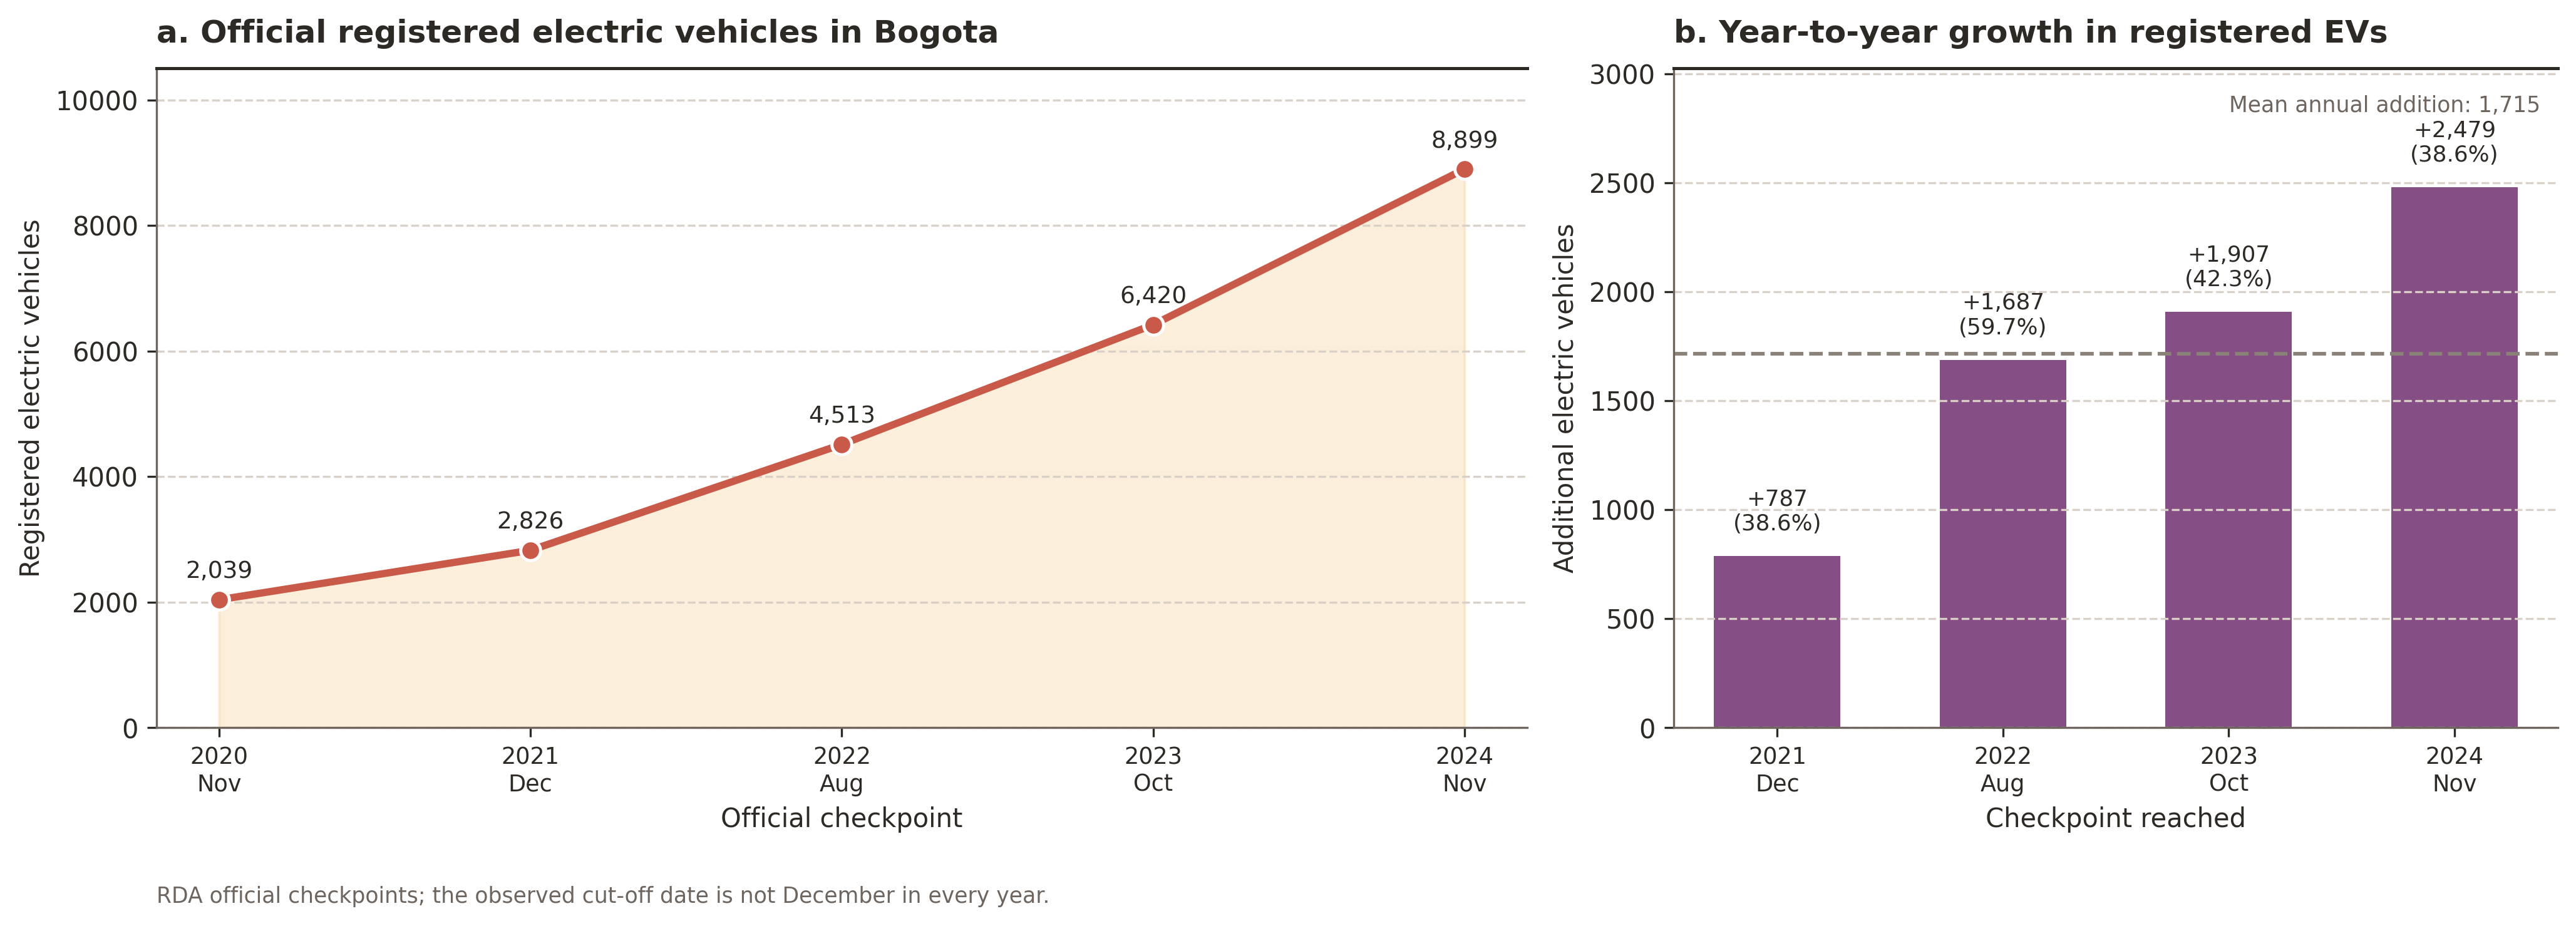
\includegraphics[width=0.98\textwidth]{figures/fig_official_ev_growth.png}
\caption{Official registration checkpoints for electric vehicles in Bogot\'a and year-to-year additions. Checkpoint dates do not always coincide with December year-end.}
\label{fig:ev_growth}
\end{figure*}

The analysis combines four data blocks: household travel survey records and mobility
profiles, EV planning baselines and venue quotas \citep{Wood2022EVIProLite},
socioeconomic and housing proxies for charging vulnerability, and road-network travel times.
Table~\ref{tab:data} summarizes each source and role.

\begin{table*}[htbp]
\centering
\caption{Core datasets and analytical roles.}
\label{tab:data}
\begin{threeparttable}
\footnotesize
\begin{tabularx}{\textwidth}{YYYY}
\toprule
Source & Role in model chain & Spatial unit & Key variables \\
\midrule
Household travel survey & Mobility features for graph learning and behavioral interpretation & Zone/time & Origin--destination flows, departure times, trip purposes \\
Socioeconomic and housing records & Vulnerability index for social-equity modeling & Zone & Income, rental tenure, apartment share, parking proxy \\
Road network or OD time matrix & Accessibility impedance and graph weights & Zone-to-zone & Travel times, generalized impedance \\
Existing EV planning framework & Exogenous quotas and benchmarking signals & City/zone & Venue quotas, baseline demand-priority references \\
\bottomrule
\end{tabularx}
\end{threeparttable}
\end{table*}

Because zone-level charger transactions are not observed in this setting, the learning target
is a survey-based proxy demand intensity rather than realized charging telemetry. The
learning stage is therefore used to recover relative spatio-temporal priorities under partial
observability, not to claim telemetry-equivalent prediction of individual charging events.
Feature construction, preprocessing, train--validation partitioning, and implementation
settings used for reproduction are documented in the blinded replication package. The
validation diagnostics reported below are computed on held-out time steps outside
$T_{\mathrm{train}}$, so the learning evaluation does not reuse the observations used to
estimate the network parameters. The main text can therefore remain focused on the
learning-to-decision chain.

\subsection{Problem framing and methodological overview}

The planning problem is to assign integer charging ports $n_{iv}$ to each zone $i \in I$ and
venue type $v \in V$ under fixed venue quotas $Q_v$, while balancing two objectives: (i)
fidelity to mobility-derived priorities and (ii) equity in effective accessibility across
urban space.

Figure~\ref{fig:workflow} summarizes the staged workflow from data assembly to policy
interpretation.

\begin{figure*}[htbp]
\centering
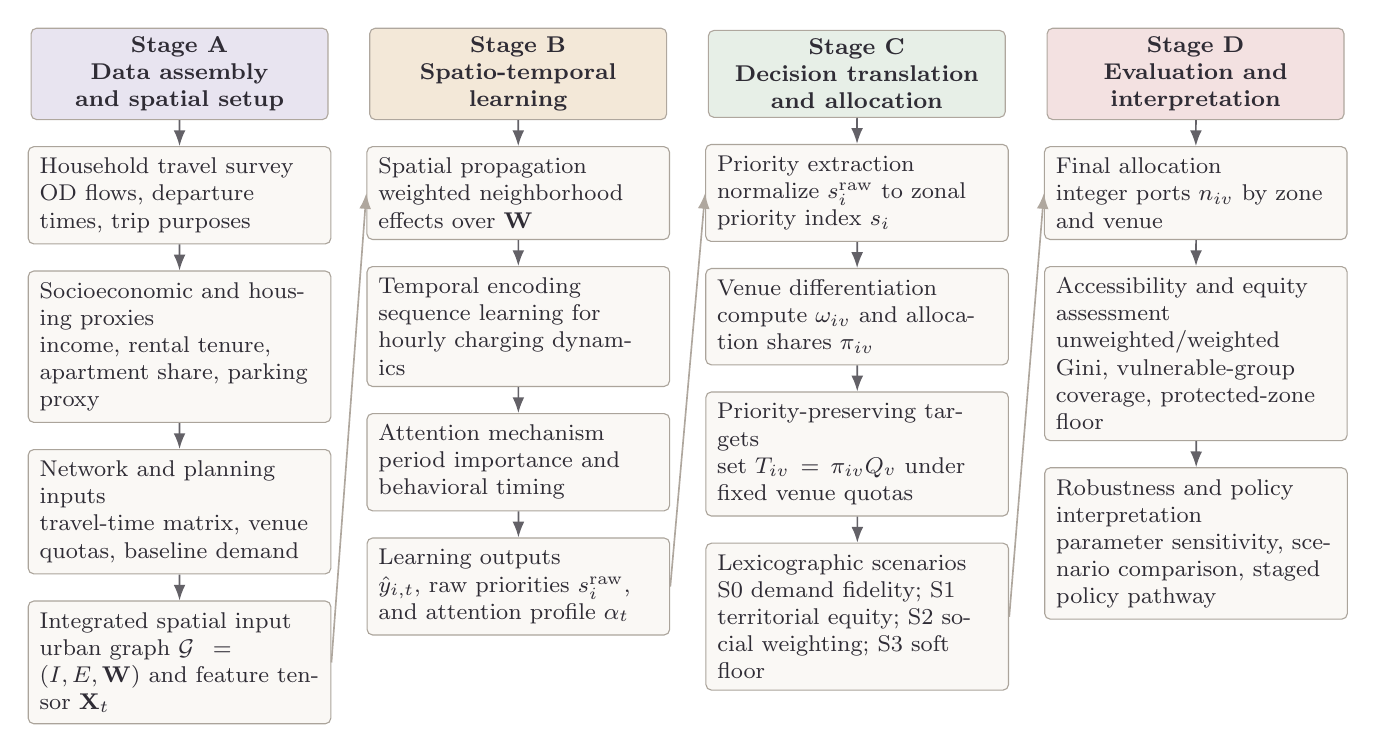
\begin{tikzpicture}[
    scale=1.03,
    transform shape,
    >=Latex,
    node distance=3.2mm and 5mm,
    stage/.style={
        draw=jtgwarmgray!95!jtgink,
        rounded corners=2pt,
        align=center,
        font=\bfseries\footnotesize,
        text=jtgink,
        text width=3.45cm,
        minimum height=9mm,
        inner sep=3pt,
    },
    stageA/.style={stage, fill=jtgmauve},
    stageB/.style={stage, fill=jtgsand},
    stageC/.style={stage, fill=jtgsage},
    stageD/.style={stage, fill=jtgblush},
    workflowbox/.style={
        draw=jtgwarmgray!92!jtgink,
        rounded corners=2pt,
        align=left,
        font=\footnotesize,
        text=jtgink,
        text width=3.45cm,
        minimum height=11mm,
        inner sep=4pt,
        fill=jtgmist
    },
    flow/.style={-Latex, semithick, draw=jtgink!75},
    stageflow/.style={-Latex, semithick, draw=jtgwarmgray!95!jtgink}
]
\node[stageA] (a0) {Stage A\\Data assembly and spatial setup};
\node[workflowbox, below=of a0] (a1) {Household travel survey\\OD flows, departure times, trip purposes};
\node[workflowbox, below=of a1] (a2) {Socioeconomic and housing proxies\\income, rental tenure, apartment share, parking proxy};
\node[workflowbox, below=of a2] (a3) {Network and planning inputs\\travel-time matrix, venue quotas, baseline demand};
\node[workflowbox, below=of a3] (a4) {Integrated spatial input\\urban graph $\mathcal{G}=(I,E,\mathbf{W})$ and feature tensor $\mathbf{X}_t$};

\node[stageB, right=of a0] (b0) {Stage B\\Spatio-temporal learning};
\node[workflowbox, below=of b0] (b1) {Spatial propagation\\weighted neighborhood effects over $\mathbf{W}$};
\node[workflowbox, below=of b1] (b2) {Temporal encoding\\sequence learning for hourly charging dynamics};
\node[workflowbox, below=of b2] (b3) {Attention mechanism\\period importance and behavioral timing};
\node[workflowbox, below=of b3] (b4) {Learning outputs\\$\hat{y}_{i,t}$, raw priorities $s_i^{\mathrm{raw}}$, and attention profile $\alpha_t$};

\node[stageC, right=of b0] (c0) {Stage C\\Decision translation and allocation};
\node[workflowbox, below=of c0] (c1) {Priority extraction\\normalize $s_i^{\mathrm{raw}}$ to zonal priority index $s_i$};
\node[workflowbox, below=of c1] (c2) {Venue differentiation\\compute $\omega_{iv}$ and allocation shares $\pi_{iv}$};
\node[workflowbox, below=of c2] (c3) {Priority-preserving targets\\set $T_{iv}=\pi_{iv}Q_v$ under fixed venue quotas};
\node[workflowbox, below=of c3] (c4) {Lexicographic scenarios\\S0 demand fidelity; S1 territorial equity; S2 social weighting; S3 soft floor};

\node[stageD, right=of c0] (d0) {Stage D\\Evaluation and interpretation};
\node[workflowbox, below=of d0] (d1) {Final allocation\\integer ports $n_{iv}$ by zone and venue};
\node[workflowbox, below=of d1] (d2) {Accessibility and equity assessment\\unweighted/weighted Gini, vulnerable-group coverage, protected-zone floor};
\node[workflowbox, below=of d2] (d3) {Robustness and policy interpretation\\parameter sensitivity, scenario comparison, staged policy pathway};

\draw[flow] (a0) -- (a1);
\draw[flow] (a1) -- (a2);
\draw[flow] (a2) -- (a3);
\draw[flow] (a3) -- (a4);

\draw[flow] (b0) -- (b1);
\draw[flow] (b1) -- (b2);
\draw[flow] (b2) -- (b3);
\draw[flow] (b3) -- (b4);

\draw[flow] (c0) -- (c1);
\draw[flow] (c1) -- (c2);
\draw[flow] (c2) -- (c3);
\draw[flow] (c3) -- (c4);

\draw[flow] (d0) -- (d1);
\draw[flow] (d1) -- (d2);
\draw[flow] (d2) -- (d3);

\draw[stageflow] (a4.east) -- (b1.west);
\draw[stageflow] (b4.east) -- (c1.west);
\draw[stageflow] (c4.east) -- (d1.west);
\end{tikzpicture}
\caption{Staged methodology from data assembly to accessibility outcomes. Stages A--D distinguish input assembly, spatio-temporal learning, translation into allocation scenarios, and evaluation/policy interpretation.}
\label{fig:workflow}
\end{figure*}

This framing keeps the main policy parameters ($\varepsilon$, $\kappa$, $\gamma$, $\beta$) explicit. The
next subsections formalize that chain.

\subsection{Graph representation and feature construction}

To encode urban interaction structure, we represent the city as a weighted graph
$\mathcal{G}=(I,E,\mathbf{W})$, where nodes are zones and edges represent feasible mobility
or accessibility interactions.

The weighted adjacency matrix is defined as:
\begin{equation}
w_{ij}=\exp(-t_{ij}/\tau),
\label{eq:adjacency}
\end{equation}
where $t_{ij}$ is network travel time from zone $i$ to zone $j$, and $\tau$ is a scale
parameter controlling distance decay. In the final implementation, this graph-based decay was
used only in the learning stage, whereas the optimization stage employed venue-specific decay
parameters $\lambda_v$ in the accessibility function.

For each zone and time step, the node-feature vector is:
\begin{equation}
\mathbf{x}_{i,t} = \left[d_{i,t}^{(1)},\ldots,d_{i,t}^{(P)},q_i^{(1)},\ldots,q_i^{(R)}\right]^\top,
\label{eq:features}
\end{equation}
where $d_{i,t}^{(p)}$ are time-varying mobility descriptors and $q_i^{(r)}$ are static zone
attributes (including socioeconomic and built-environment factors). Here $P$ and $R$ denote
the numbers of time-varying and static features, respectively. Stacking all zones gives
$\mathbf{X}_t\in\mathbb{R}^{|I|\times(P+R)}$.

To keep the main text focused on model logic, notation used in Sections 3.3--3.5 is
summarized in Supplementary Appendix A.

This representation is required for the next step, where spatial propagation and temporal
encoding jointly extract decision-relevant mobility signals.

\subsection{Spatio-temporal GNN model}

Given $\mathcal{G}$ and $\mathbf{X}_t$, spatial dependence is modeled through message passing:
\begin{equation}
\mathbf{h}_{i,t}^{(l+1)} = \sigma\left(
\mathbf{W}_s^{(l)}\mathbf{h}_{i,t}^{(l)} + \sum_{j\in\mathcal{N}(i)} w_{ij}\mathbf{U}_s^{(l)}\mathbf{h}_{j,t}^{(l)}
\right),
\label{eq:spatial_layer}
\end{equation}
where $\mathcal{N}(i)$ denotes the neighbors of zone $i$, $l=1,\ldots,L$ indexes the spatial
message-passing layers, $\mathbf{W}_s^{(l)}$ and $\mathbf{U}_s^{(l)}$ are trainable weight
matrices, and $\sigma(\cdot)$ is a nonlinear activation.

Temporal dynamics are then captured by a recurrent update:
\begin{equation}
\mathbf{g}_{i,t}=\mathrm{GRU}\left(\mathbf{h}_{i,t}^{(L)},\mathbf{g}_{i,t-1}\right),
\label{eq:temporal_layer}
\end{equation}
and the demand signal is read out as:
\begin{equation}
\hat{y}_{i,t}=f_{\mathrm{out}}(\mathbf{g}_{i,t}).
\label{eq:readout}
\end{equation}
where $f_{\mathrm{out}}(\cdot)$ is the output head of the network.

To identify behaviorally relevant periods, we compute temporal attention weights:
\begin{equation}
\alpha_t = \frac{\exp\left(\mathbf{q}^\top\tanh(\mathbf{W}_a\mathbf{r}_t)\right)}
{\sum_{\tau\in T}\exp\left(\mathbf{q}^\top\tanh(\mathbf{W}_a\mathbf{r}_{\tau})\right)},
\qquad
\mathbf{r}_t=\frac{1}{|I|}\sum_{i\in I}\mathbf{g}_{i,t},
\label{eq:attention}
\end{equation}
where $\mathbf{r}_t$ is the mean latent representation at time $t$, and $\mathbf{q}$ and
$\mathbf{W}_a$ are trainable attention parameters. We then aggregate zone-level raw
priority as:
\begin{equation}
s_i^{\mathrm{raw}}=\sum_{t\in T}\alpha_t\hat{y}_{i,t}.
\label{eq:raw_priority}
\end{equation}

Model parameters are estimated by minimizing:
\begin{equation}
\mathcal{L}_{\mathrm{GNN}}=
\frac{1}{|I||T_{\mathrm{train}}|}
\sum_{t\in T_{\mathrm{train}}}\sum_{i\in I}(\hat{y}_{i,t}-y_{i,t})^2.
\label{eq:loss}
\end{equation}
where $T_{\mathrm{train}}\subseteq T$ is the subset of time steps used for training.

In this paper, the learning model is treated as a priority-extraction component within a
broader planning chain. Predictive diagnostics are reported for transparency, but the main
substantive claim of the article concerns the auditable translation from learned signals to
allocation rules rather than algorithmic dominance over simpler forecasting baselines.

Equation~\eqref{eq:spatial_layer} captures spatial spillovers. Equation~
\eqref{eq:temporal_layer} captures temporal dependence. Equations~
\eqref{eq:attention}--\eqref{eq:raw_priority} convert predictions into interpretable
priority signals. This output is the direct input to the allocation model in the next
subsection.

\subsection{Priority extraction and behavioral interpretation}

The optimization model requires normalized and venue-specific signals rather than raw
predictions. We therefore normalize raw priorities into $[0,1]$:
\begin{equation}
s_i=\frac{s_i^{\mathrm{raw}}-\min_{k\in I} s_k^{\mathrm{raw}}}
{\max_{k\in I} s_k^{\mathrm{raw}}-\min_{k\in I} s_k^{\mathrm{raw}}}.
\label{eq:normalized_priority}
\end{equation}
If the raw-priority range were to collapse to zero, the implementation would revert to a
uniform zonal priority vector; this safeguard was not triggered in the reproduced run.

Venue-specific weights are extracted by aggregating attention-weighted predictions over
venue-relevant periods $T_v$:
\begin{equation}
\omega_{iv}=\frac{\sum_{t\in T_v}\alpha_t\hat{y}_{i,t}}
{\sum_{v'\in V}\sum_{t\in T_{v'}}\alpha_t\hat{y}_{i,t}}.
\label{eq:venue_weights}
\end{equation}
Here $T_v\subseteq T$ denotes the venue-relevant time window for venue type $v$; in the
empirical implementation these windows are mutually exclusive and correspond to residential,
work, and public-service periods. If the denominator in Eq.~\eqref{eq:venue_weights} were
zero for a zone, the implementation would assign uniform venue weights; this safeguard was
not triggered in the reproduced run.

These quantities define optimization shares:
\begin{equation}
\pi_{iv}=\frac{s_i\omega_{iv}}{\sum_{k\in I}s_k\omega_{kv}},
\qquad
T_{iv}=\pi_{iv}Q_v.
\label{eq:targets}
\end{equation}

Equation~\eqref{eq:normalized_priority} preserves relative ranking across zones.
Equation~\eqref{eq:venue_weights} maps temporal behavior into venue differentiation.
Equation~\eqref{eq:targets} translates learning outputs into target allocations. This is the
explicit GNN $\to$ optimization bridge used in Section 3.6.

\subsection{Two-stage lexicographic optimization model}

The allocation model is solved lexicographically. First, it minimizes deviation from
priority-preserving targets $T_{iv}$. Second, it minimizes accessibility inequality while
allowing only bounded deterioration in priority fidelity.

Optimization notation is summarized in Supplementary Appendix B.
In scenarios S1--S3, the lower-level problem is solved over the same feasible set defined by
Eqs.~\eqref{eq:upper_abs1}--\eqref{eq:upper_domain}; the lower-level constraints introduced
below are added to those upper-level requirements rather than replacing them.

Social vulnerability is defined as:
\begin{equation}
\nu_i = \frac{\sum_{m\in M} \eta_m z_{im} - \min_{k\in I}\sum_{m\in M} \eta_m z_{km}}
{\max_{k\in I}\sum_{m\in M} \eta_m z_{km} - \min_{k\in I}\sum_{m\in M} \eta_m z_{km}}.
\label{eq:vulnerability}
\end{equation}

Accessibility is computed as:
\begin{equation}
A_i = \sum_{v\in V}\omega_{iv}\sum_{j\in I}\exp(-t_{ij}/\lambda_v)n_{jv}.
\label{eq:accessibility}
\end{equation}

\paragraph{Upper level (priority fidelity).}
\begin{equation}
\min U=\sum_{i\in I}\sum_{v\in V}u_{iv}
\label{eq:upper_obj}
\end{equation}
subject to
\begin{align}
u_{iv} &\ge n_{iv}-T_{iv} && \forall i\in I,\forall v\in V, \label{eq:upper_abs1} \\
u_{iv} &\ge T_{iv}-n_{iv} && \forall i\in I,\forall v\in V, \label{eq:upper_abs2} \\
\sum_{i\in I}n_{iv} &= Q_v && \forall v\in V, \label{eq:upper_quota} \\
n_{iv} &\in \mathbb{Z}_{+},\; u_{iv}\ge 0 && \forall i\in I,\forall v\in V. \label{eq:upper_domain}
\end{align}

The objective function minimizes total deviation from GNN-derived target allocations.
Constraint~\eqref{eq:upper_abs1} and Constraint~\eqref{eq:upper_abs2} linearize absolute
deviations. Constraint~\eqref{eq:upper_quota} enforces venue-specific quota conservation.
Constraint~\eqref{eq:upper_domain} defines variable domains.

\paragraph{Lower level (equity objective with bounded fidelity loss).}
Let $U^{\star}$ be the optimum of Eq.~\eqref{eq:upper_obj}. Accessibility-gap linearization is:
\begin{align}
z_{ij} &\ge A_i-A_j && \forall i<j, \label{eq:gap1} \\
z_{ij} &\ge A_j-A_i && \forall i<j, \label{eq:gap2} \\
z_{ij} &\ge 0 && \forall i<j. \label{eq:gap3}
\end{align}

The unweighted and socially weighted equity objectives are, respectively:
\begin{align}
\min E_{\mathrm{U}} &= \sum_{i<j}z_{ij}, \label{eq:lower_unweighted} \\
\min E_{\mathrm{W}} &= \sum_{i<j}\bar{\nu}_{ij}z_{ij}, \qquad
\bar{\nu}_{ij}=1+\kappa\frac{\nu_i+\nu_j}{2}. \label{eq:lower_weighted}
\end{align}

Near-optimal coupling is imposed as:
\begin{align}
\sum_{i\in I}\sum_{v\in V}u_{iv} &\le (1+\varepsilon)U^{\star}. \label{eq:near_opt}
\end{align}

For the minimum-service scenario, the protected set $\mathcal{V}^{H}$ is defined as the top
15\% of zones in the vulnerability distribution, operationalized in the reproduced run as the
22 highest-ranked zones under $\nu_i$ ($\lceil 0.15|I|\rceil$ with $|I|=142$), and the
accessibility floor is implemented as a soft constraint:
\begin{align}
A_i + d_i &\ge \underline{A} && \forall i\in \mathcal{V}^{H}, \label{eq:soft_floor} \\
d_i &\ge 0 && \forall i\in \mathcal{V}^{H}. \label{eq:soft_floor_nonneg}
\end{align}

In the empirical implementation, the floor is calibrated from the lower tail of the socially
weighted baseline solution:
\begin{equation}
\underline{A}=\gamma\,q_{0.10}\!\left(\{A_i^{S2}: i\in \mathcal{V}^{H}\}\right),
\label{eq:floor_calibration}
\end{equation}
where, after sorting $\{A_i^{S2}: i\in \mathcal{V}^{H}\}$ in ascending order,
$q_{0.10}(\cdot)$ denotes the empirical order-statistic percentile
$A_{(\lceil 0.10|\mathcal{V}^{H}|\rceil)}^{S2,H}$ on that discrete protected-set sample, and
$0<\gamma\le 1$ is a floor-relaxation factor.

In scenario S3, the soft-floor shortfalls are penalized jointly with weighted accessibility
inequality. Let $\beta>0$ denote the shortfall penalty. The S3 objective is:
\begin{equation}
\min E_{\mathrm{F}}=\sum_{i<j}\bar{\nu}_{ij}z_{ij}+\beta\sum_{i\in \mathcal{V}^{H}} d_i.
\label{eq:lower_weighted_floor}
\end{equation}
This formulation preserves the socially weighted structure of S2 while introducing an
explicit lower-tail service guarantee.

For reporting, the inequality and coverage metrics are computed ex post from the realized
accessibility vector $A_i$ rather than read directly from the lower-level objective value.
Let $\mathcal{V}^{Q}\subset I$ denote the most vulnerable quartile of zones (the top 25\% of
the $\nu_i$ distribution), operationalized in the reproduced run as the 36 highest-ranked
zones under $\nu_i$ ($\lceil 0.25|I|\rceil$ with $|I|=142$). The reported
vulnerable-quartile share and vulnerable-zone coverage are:
\begin{align}
S^{Q} &= \frac{\sum_{i\in \mathcal{V}^{Q}} A_i}{\sum_{i\in I} A_i},
\label{eq:vulnerable_quartile_share} \\
C^{15} &= \frac{1}{|\mathcal{V}^{Q}|}\sum_{i\in \mathcal{V}^{Q}} c_i^{15},
\label{eq:coverage_threshold_metric} \\
c_i^{15} &= \mathbf{1}\!\left[\exists j\in I:\ t_{ij}\le 15,\ \sum_{v\in V} n_{jv}>0\right].
\nonumber
\end{align}
The unweighted accessibility Gini sorts $\{A_i\}_{i\in I}$ into ascending order
$A_{(1)}\le \cdots \le A_{(|I|)}$, defines cumulative totals
$C_k=\sum_{r=1}^{k}A_{(r)}$, and computes:
\begin{equation}
G=\frac{|I|+1-2\sum_{k=1}^{|I|} C_k/C_{|I|}}{|I|}.
\label{eq:accessibility_gini}
\end{equation}
The vulnerability-weighted accessibility Gini uses zone weights $1+\nu_i$:
\begin{align}
G_{\mathrm{W}} &=
\frac{\sum_{i\in I}\sum_{j\in I}(1+\nu_i)(1+\nu_j)|A_i-A_j|}
{2\mu_{\nu}\left(\sum_{i\in I}(1+\nu_i)\right)^2},
\label{eq:weighted_accessibility_gini} \\
\mu_{\nu} &=
\frac{\sum_{i\in I}(1+\nu_i)A_i}{\sum_{i\in I}(1+\nu_i)}.
\nonumber
\end{align}
Figure~\ref{fig:lorenz_curves} uses the corresponding Lorenz diagnostics after sorting zones
by $A_i$; in the weighted case, the horizontal axis is the cumulative share of
$\sum_i(1+\nu_i)$ and the vertical axis is the cumulative share of
$\sum_i(1+\nu_i)A_i$.

The objective functions minimize accessibility inequality in unweighted or
vulnerability-weighted form. Constraint~\eqref{eq:near_opt} links equity improvements to an
explicit bound on priority-fidelity loss. Constraints~\eqref{eq:soft_floor} and~
\eqref{eq:soft_floor_nonneg} define a soft minimum-service guarantee for high-vulnerability
zones, allowing limited shortfalls when a hard floor would make the model infeasible.

This lexicographic design operationalizes the full chain of the paper: learned priorities set
the target, and optimization transforms that target into socially evaluated allocations.

\subsection{Solution strategy and implementation}

The model is implemented in Pyomo. Stage A trains the ST-GNN and exports
${s_i,\omega_{iv},\pi_{iv},T_{iv}}$. Stage B solves the two-stage lexicographic allocation
model as a mixed-integer linear program on NEOS using CPLEX in the final experimental runs.
The upper-level problem is solved first to obtain $U^{\star}$, after which lower-level
equity scenarios are solved under the near-optimality constraint in
Eq.~\eqref{eq:near_opt}.

Scenario definitions are shown in Table~\ref{tab:scenarios}. In the final implementation,
the accessibility kernel used $\lambda_{\mathrm{res}}=15$, $\lambda_{\mathrm{work}}=25$, and
$\lambda_{\mathrm{pub}}=10$ minutes. S1 used $\varepsilon=0.03$, while S2 and S3 used
$\varepsilon=0.08$. The socially weighted objective used $\kappa=4.0$. The protected set in
S3 was defined as the top 15\% of zones in the vulnerability distribution, implemented as the
22 highest-ranked zones under $\nu_i$, and the soft floor was calibrated using
$\gamma=0.95$ and the empirical 10th percentile of S2 accessibility in that protected set.
The shortfall penalty in S3 was set to $\beta=100$. For reporting, the top-quartile set
$\mathcal{V}^{Q}$ used in Eqs.~\eqref{eq:vulnerable_quartile_share}--
\eqref{eq:coverage_threshold_metric} is distinct from the top-15\% protected set
$\mathcal{V}^{H}$ used only in S3 and is implemented as the 36 highest-ranked zones under
$\nu_i$. In the reproduced run, the S3 penalty term does not change the allocation
relative to S2, even though one protected zone retains a positive shortfall.
Accordingly, S3 is interpreted as a diagnostic soft-floor robustness check rather than as a
substantively distinct redistribution outcome.

Performance is assessed with (i) priority-fidelity indicators, (ii) unweighted and weighted
accessibility inequality, (iii) vulnerable-group coverage over the top vulnerability quartile
within a 15-minute threshold, and (iv) robustness to decay, weighting, and policy
assumptions. This metric design directly structures Section 4.

\begin{table*}[htbp]
\centering
\caption{Policy scenarios used in the lexicographic allocation model.}
\label{tab:scenarios}
\begin{threeparttable}
\footnotesize
\begin{tabularx}{\textwidth}{Z Y Z Z Y}
\toprule
Scenario & Policy role & $\varepsilon$ & $\kappa$ & Floor specification \\
\midrule
S0 & Priority-matching baseline & 0.00 & --- & None \\
S1 & Equity relaxation without vulnerability weights & 0.03 & 0.0 & None \\
S2 & Socially weighted equity scenario & 0.08 & 4.0 & None \\
S3 & Diagnostic soft-floor robustness check & 0.08 & 4.0 & Soft floor on top 15\% protected set; $\gamma=0.95$; $\beta=100$ \\
\bottomrule
\end{tabularx}
\begin{tablenotes}[flushleft]
\footnotesize
\item Notes: Relative fidelity losses versus S0 are 0.0\%, 3.0\%, 8.0\%, and 8.0\%,
respectively. Coverage of vulnerable UTAMs within 15 minutes is $C^{15}$ from
Eq.~\eqref{eq:coverage_threshold_metric}, evaluated on the top vulnerability quartile
$\mathcal{V}^{Q}$; this reporting set is distinct from the top-15\% protected set
$\mathcal{V}^{H}$ used only in S3. In the reproduced run, S3 reproduces the S2 allocation;
the soft-floor penalty does not change $n_{iv}$ relative to S2 and therefore acts as a
diagnostic check rather than as an additional redistributive stage.
\end{tablenotes}
\end{threeparttable}
\end{table*}

\section{Results}

The results are presented in the following order: empirical context, socio-spatial
learning outputs, scenario allocations, distributional equity, and a compact policy
trade-off interpretation.

\subsection{Socio-spatial learning context and temporal attention}

The ST-GNN produces a differentiated spatial priority surface rather than a uniform citywide
demand map. Figure~\ref{fig:social_context} shows that learned priority and social
vulnerability only partially overlap: high-priority areas concentrate in a limited subset of
the metropolitan footprint, whereas vulnerability is more diffusely distributed across the
consolidated urban core. The protected geography used in S3 is likewise compact and
localized, which makes targeted vulnerability-sensitive reallocation possible under fixed
quotas.

Temporal structure is equally important. Figure~\ref{fig:attention_profile} shows that the
learned attention profile is strongest in the earliest hours of the day and then flattens
through work and public-service windows. When disaggregated by social vulnerability,
high-vulnerability zones receive relatively more weight in the first hours, whereas
low-vulnerability zones retain a flatter daytime profile. Additional learning diagnostics
report a best validation MAE of 10.333 and an attention-concentration index of 0.00257,
indicating that attention remains diffuse rather than collapsing onto a single time slice.
The MAE should be interpreted in the scale of the proxy-demand target rather than as a direct
measure of observed charger transactions.

\begin{figure*}[htbp]
\centering
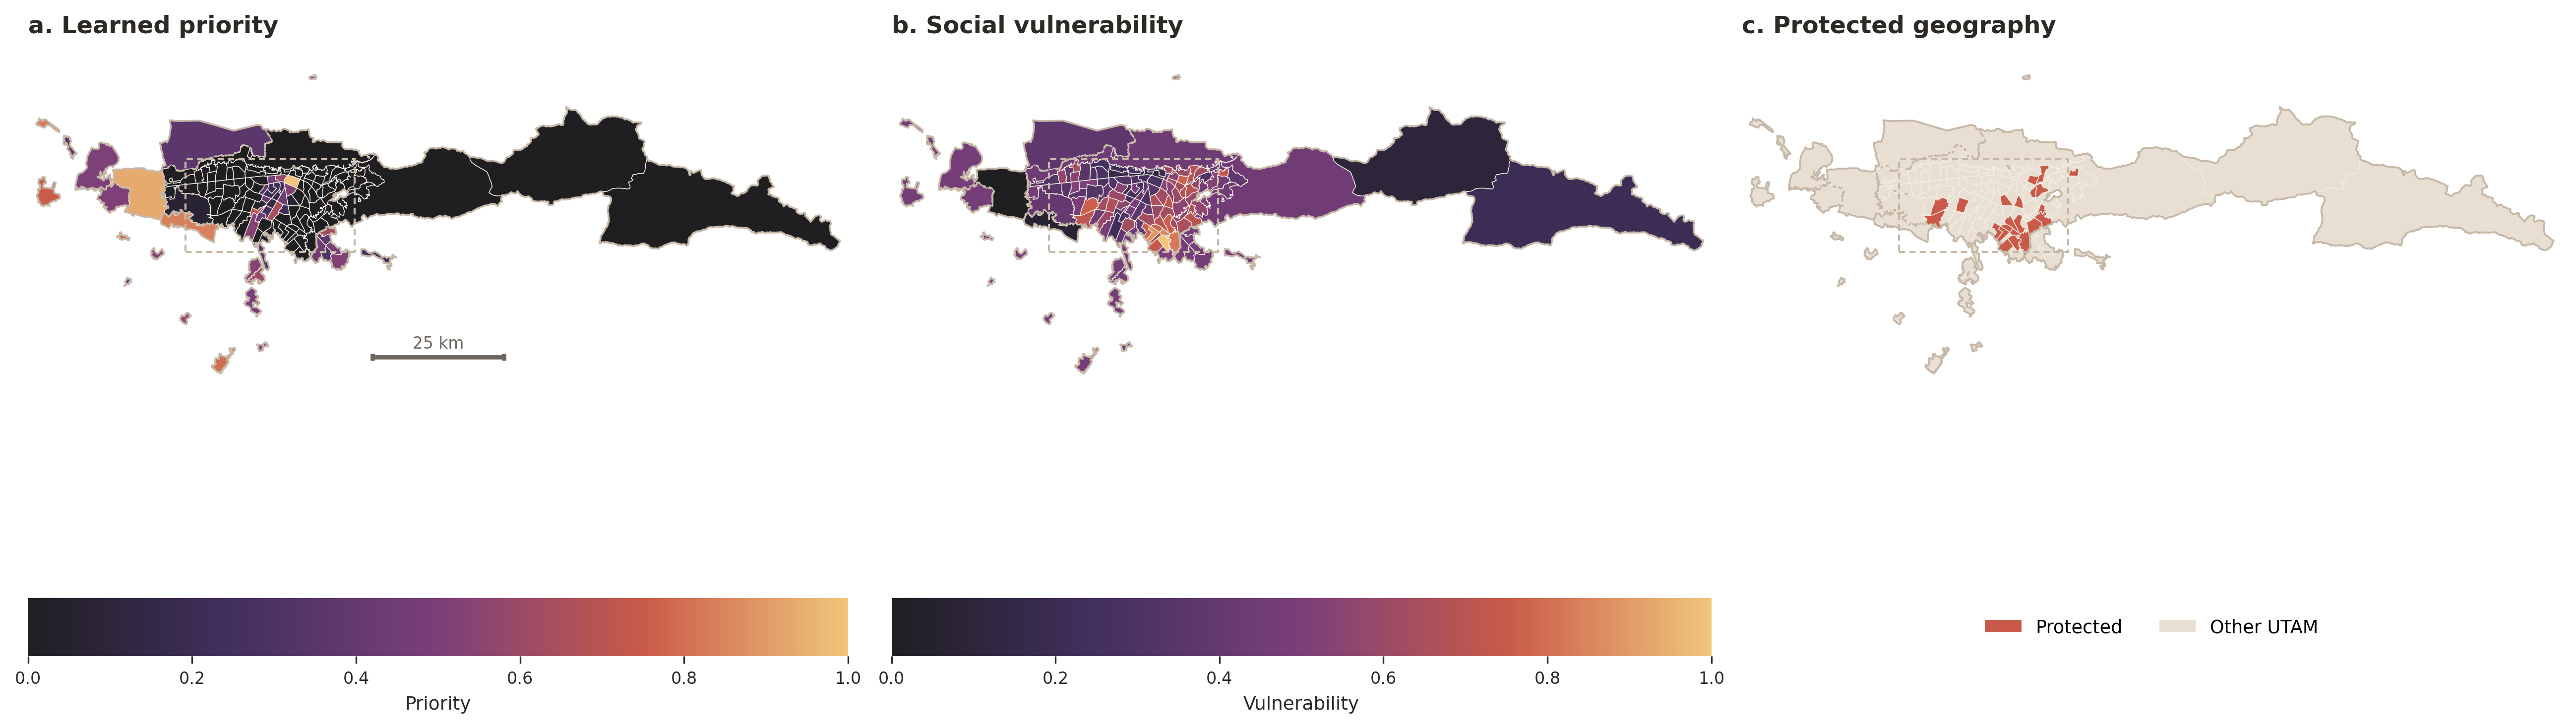
\includegraphics[width=0.98\textwidth]{figures/fig_social_context_panels.png}
\caption{Socio-spatial inputs to the allocation stage: learned zonal priority, social vulnerability, and the protected geography used in the soft-floor scenario.}
\label{fig:social_context}
\end{figure*}

\begin{figure*}[htbp]
\centering
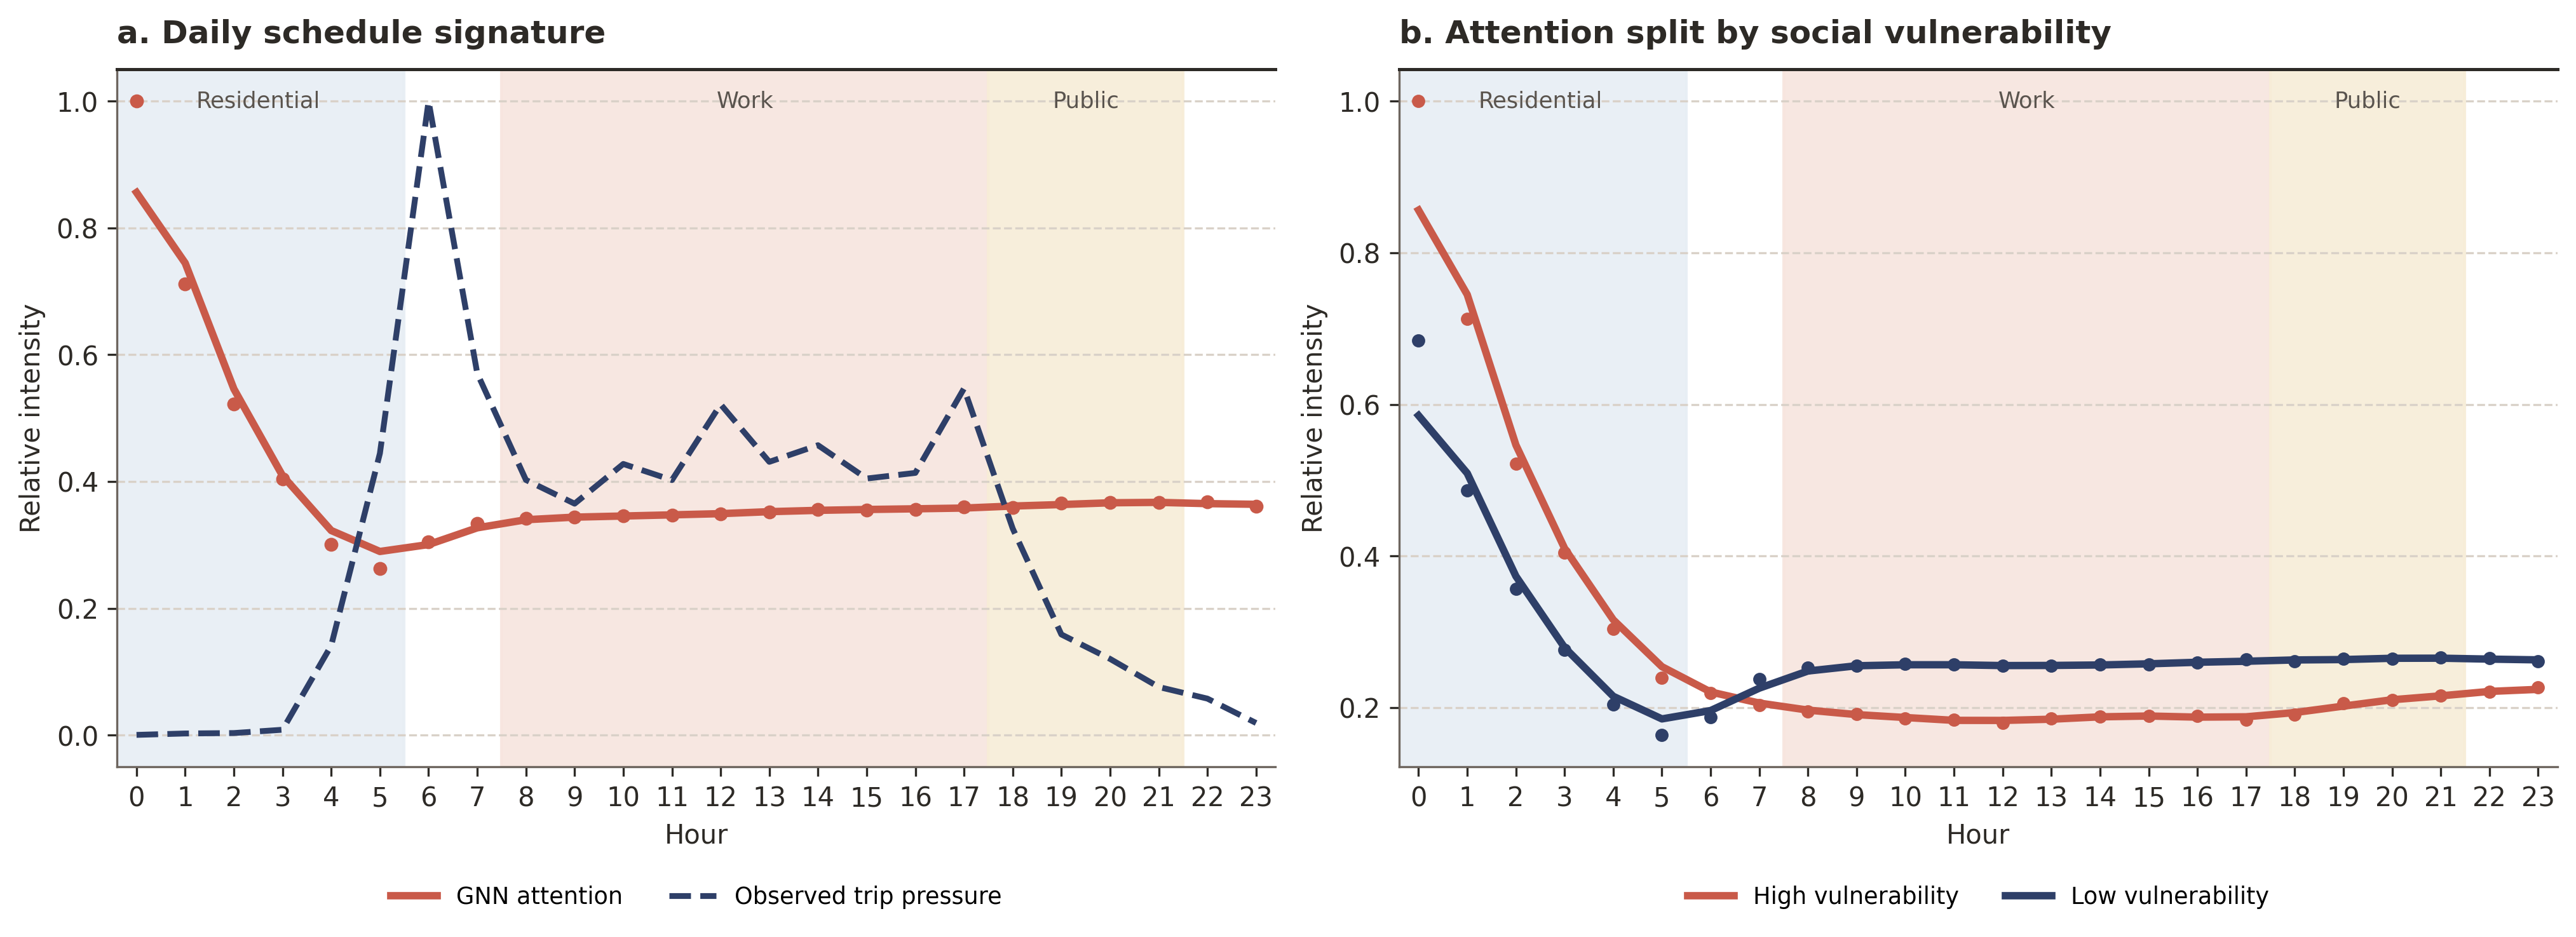
\includegraphics[width=0.98\textwidth]{figures/fig_attention_profile.png}
\caption{Temporal attention structure from the ST-GNN. Panel (a) compares hourly GNN attention with observed trip pressure across residential, work, and public windows; panel (b) splits the attention profile by social vulnerability.}
\label{fig:attention_profile}
\end{figure*}

\subsection{Scenario allocations and reallocation logic}

Figure~\ref{fig:allocation_composite} shows that all four scenarios preserve the broad
metropolitan structure of the learned allocation while redistributing ports within the
consolidated urban core. Rank alignment between learned priority and installed ports remains
high across scenarios, with Spearman correlations of 0.922119 in S0, 0.916699 in S1, and
0.910472 in both S2 and S3. The absolute-deviation objective rises from 62.828438 in S0 to
64.713291 in S1 and 67.854713 in S2/S3, implying relative fidelity losses of 3.0\% and
8.0\%, respectively. Under fixed venue quotas and integer port assignments, these numerical
changes are necessarily incremental, so even one-port reallocations should be interpreted as
localized policy moves rather than as large system-wide redistributions.

The socially weighted scenario changes the allocation in 10 zones relative to S1. These are
sparse, local reallocations---five one-port gains offset by five one-port losses---rather
than a citywide reshuffling. Figure~\ref{fig:allocation_net_change} makes this explicit. S3
is visually identical to S2 because the soft-floor term is non-binding in the reproduced run.
The gains and losses form a compact cluster of spatially adjacent UTAMs in the consolidated
inner urban area rather than a center--periphery inversion, which points to corridor-level
rebalancing among neighboring zones with similar demand intensity but different vulnerability
profiles.

\begin{figure*}[htbp]
\centering
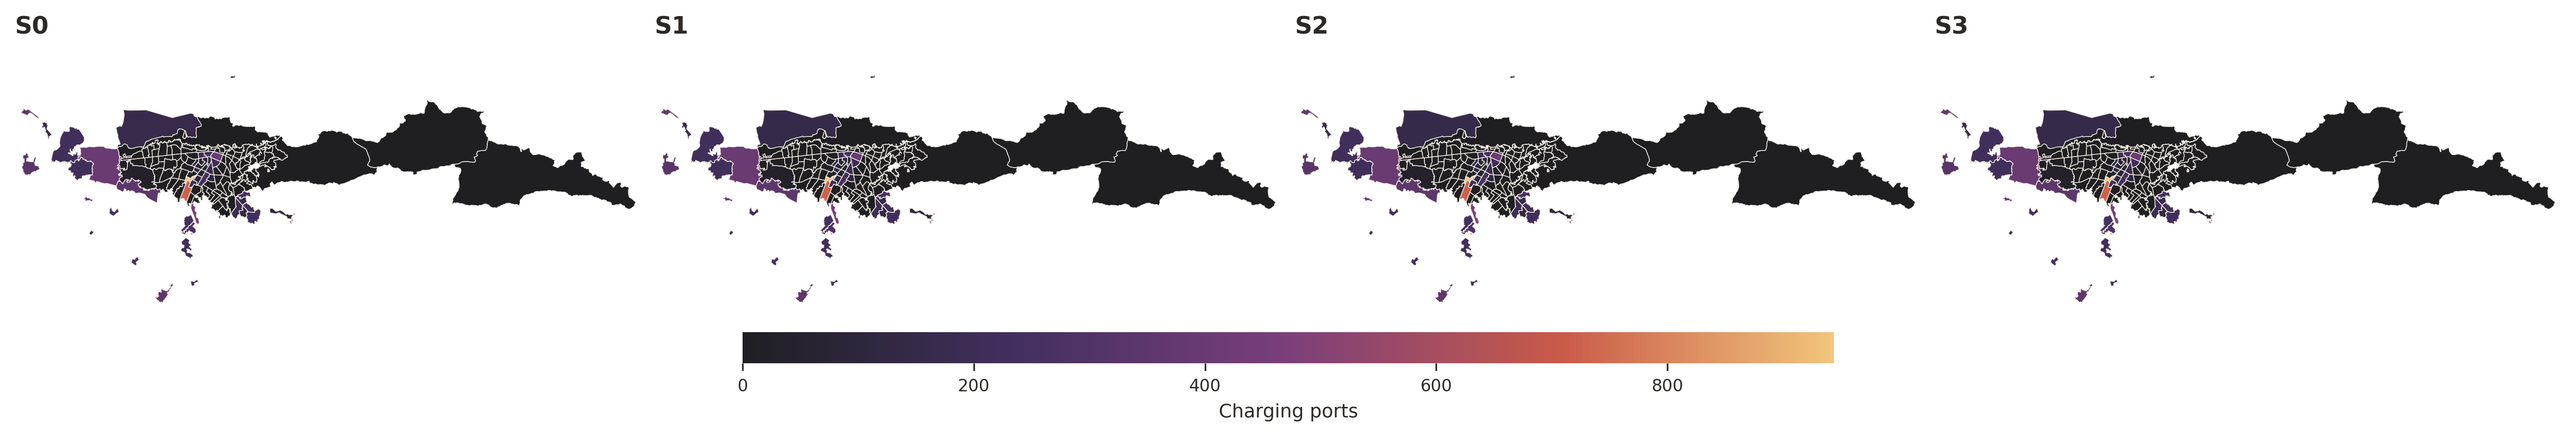
\includegraphics[width=0.98\textwidth]{figures/fig_allocation_composite.png}
\caption{Scenario allocation maps for S0--S3. The soft-floor scenario S3 is visually identical to S2 because the floor term is non-binding in the reproduced solution.}
\label{fig:allocation_composite}
\end{figure*}

\begin{figure*}[htbp]
\centering
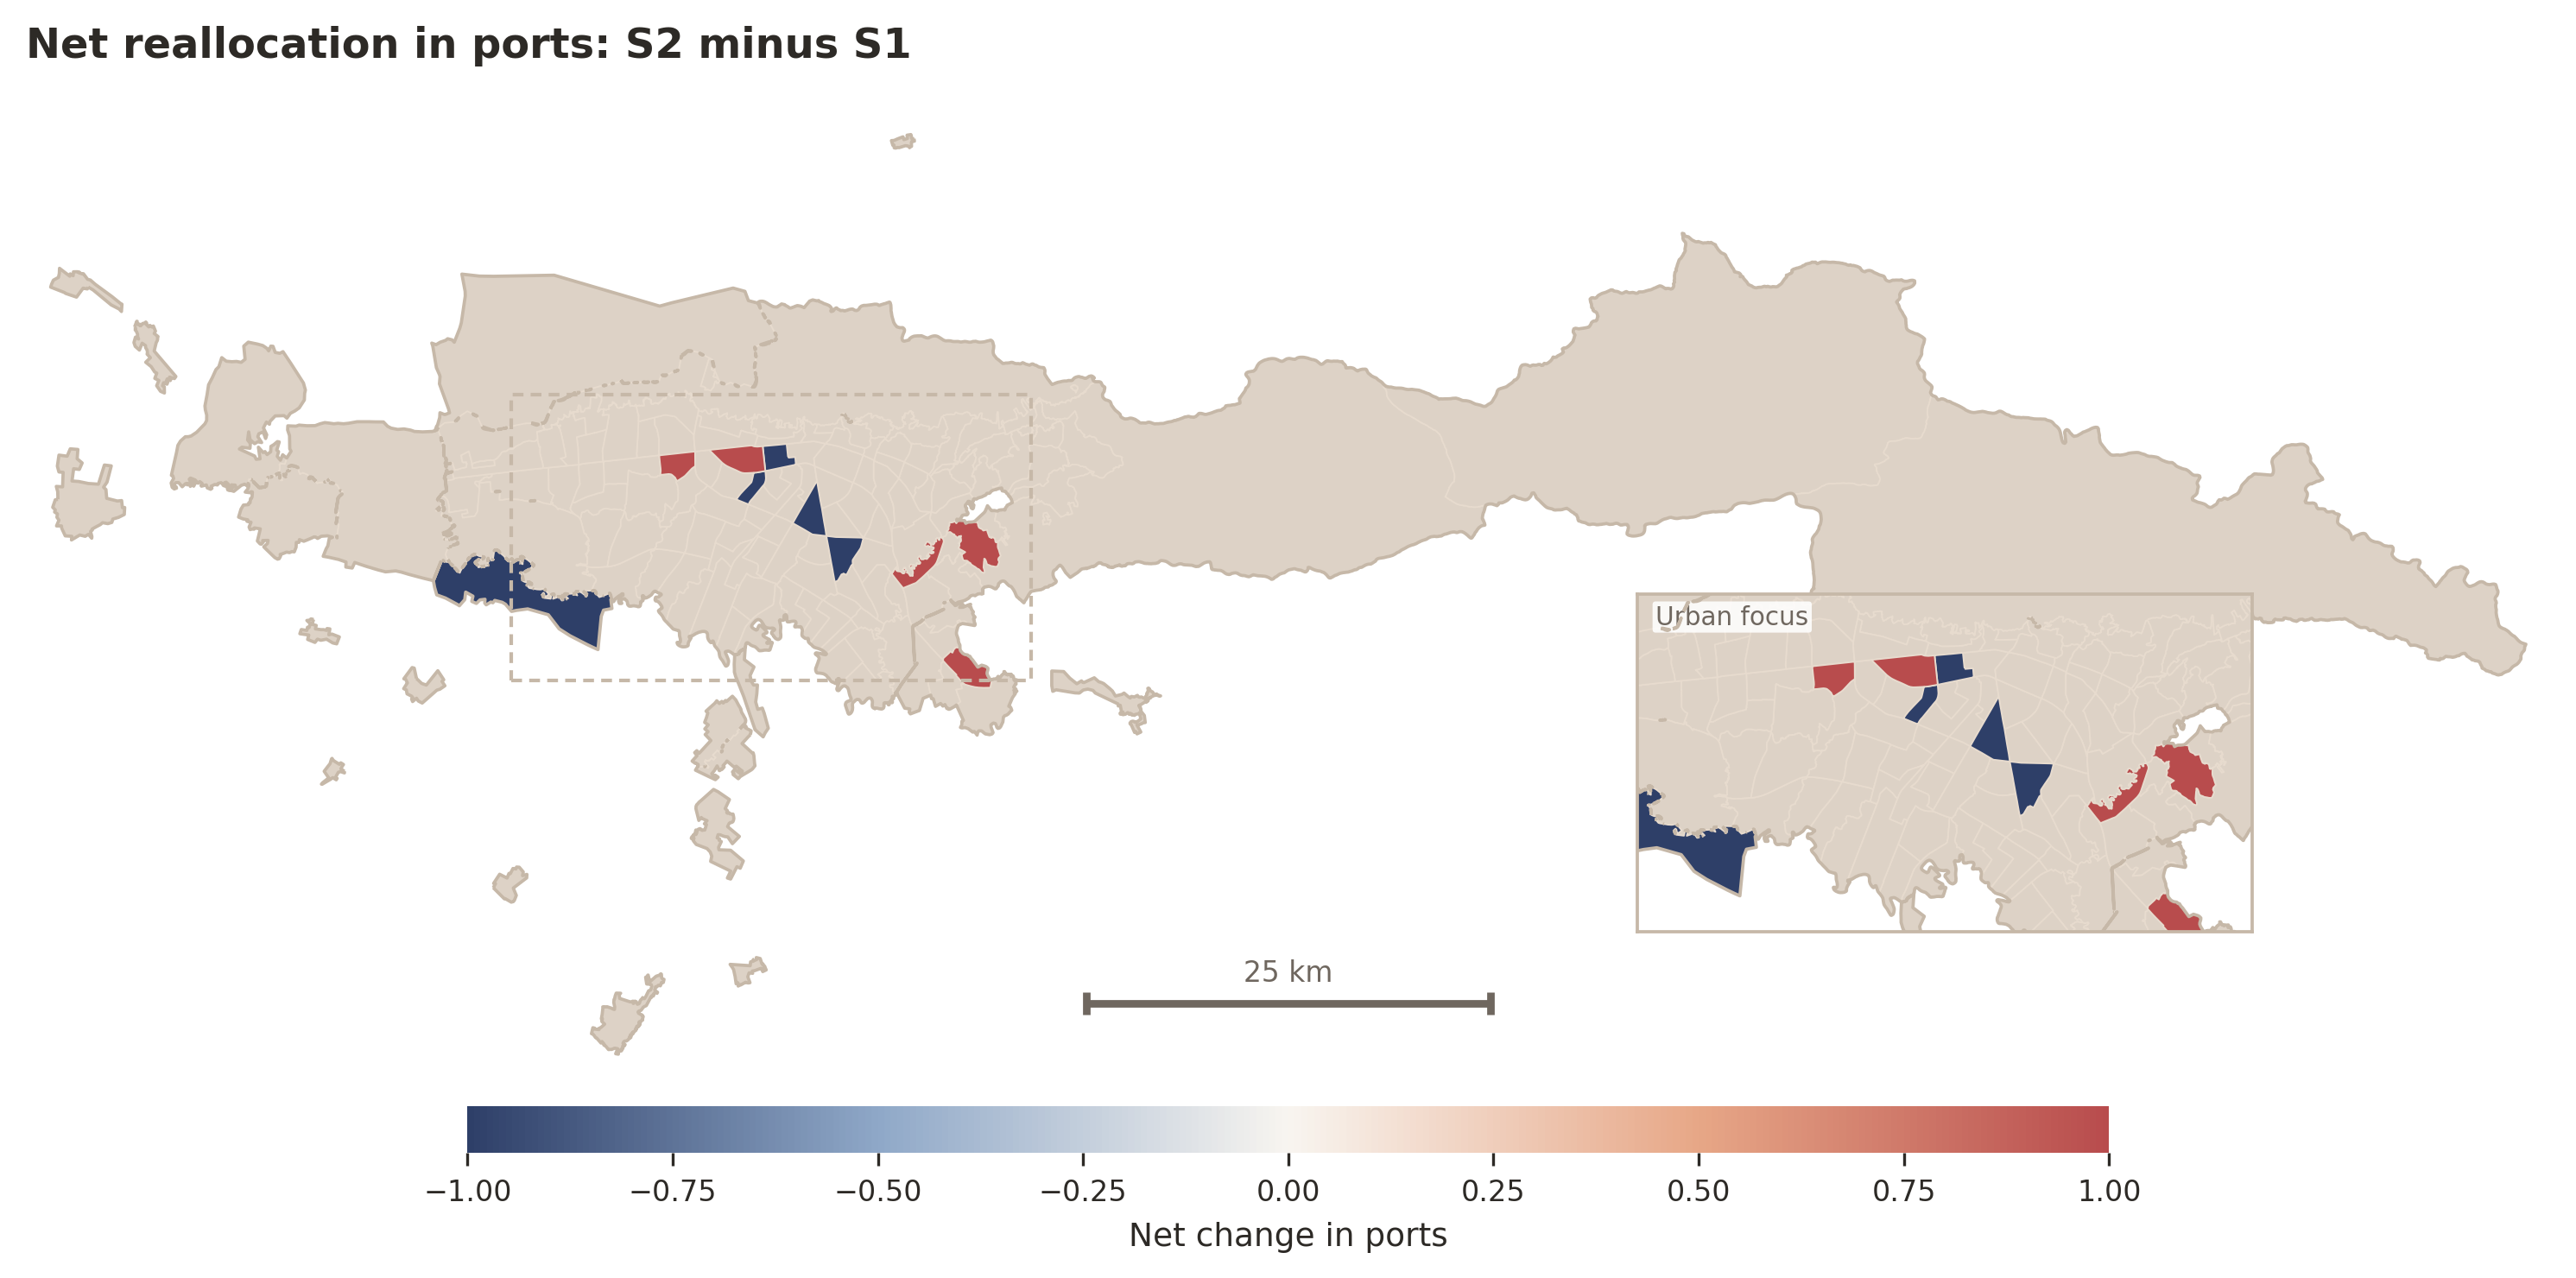
\includegraphics[width=0.98\textwidth]{figures/fig_net_change_S2_minus_S1.png}
\caption{Net reallocation in charging ports under socially weighted equity relative to territorial equalization (S2 minus S1). Positive values indicate one-port gains and negative values indicate one-port losses.}
\label{fig:allocation_net_change}
\end{figure*}

\subsection{Equity outcomes and policy trade-offs}

Table~\ref{tab:equity_metrics} shows that socially weighted allocation improves the headline
inequality and coverage indicators relative to both S0 and S1. Relative to territorial
equalization (S1), the
vulnerability-weighted accessibility Gini falls from 0.197041 to 0.196896, the unweighted
Gini falls from 0.201248 to 0.201111, and vulnerable-zone coverage within 15 minutes rises
from 86.11\% to 88.89\%. Mean accessibility in the protected high-vulnerability set changes
only slightly (from 410.324 to 410.265), indicating that the equity gains come mainly from
lower-tail rebalancing rather than large average increases. In relative terms, the reduction
in the weighted Gini is small, which is consistent with the fact that the feasible policy
move set is restricted to a limited number of integer reallocations under fixed quotas.

S3 does not produce additional allocational redistribution because it coincides with S2. The
calibrated floor equals 287.140880 accessibility units, and 95.45\% of protected zones
already meet that threshold under the reproduced solution. The remaining total shortfall is
5.199 accessibility units, so the penalty term operates as a diagnostic safeguard without
altering the final allocation in this run.

The slight decline in the share of accessibility captured by the most vulnerable quartile does
not contradict the improvement in the weighted Gini. The quartile-share indicator is an
aggregate concentration measure, whereas the lower-level objective directly targets pairwise
dispersion and lower-tail shortfalls. In this reproduced run, the socially weighted scenario
improves the lower tail mainly through rebalancing within and around vulnerable areas rather
than by increasing the aggregate accessibility share captured by the vulnerable quartile as a
whole.

\begin{table*}[htbp]
\centering
\caption{Accessibility and equity metrics by scenario.}
\label{tab:equity_metrics}
\begin{threeparttable}
\footnotesize
\begin{tabularx}{\textwidth}{Y Z Z Z Z}
\toprule
Metric & S0 & S1 & S2 & S3 \\
\midrule
Accessibility Gini (unweighted) & 0.2015 & 0.2012 & 0.2011 & 0.2011 \\
Accessibility Gini (vulnerability-weighted) & 0.1972 & 0.1970 & 0.1969 & 0.1969 \\
Share of accessibility captured by most vulnerable quartile & 0.2725 & 0.2724 & 0.2723 & 0.2723 \\
Coverage within 15 minutes for vulnerable UTAMs & 0.7778 & 0.8611 & 0.8889 & 0.8889 \\
Mean accessibility in protected set $\mathcal{V}^{H}$ & 410.68 & 410.32 & 410.26 & 410.26 \\
\bottomrule
\end{tabularx}
\begin{tablenotes}[flushleft]
\footnotesize
\item Notes: In S3, the protected-set floor is calibrated at 287.14 accessibility units. The vulnerable-quartile share is $S^{Q}$ from Eq.~\eqref{eq:vulnerable_quartile_share}, coverage is $C^{15}$ from Eq.~\eqref{eq:coverage_threshold_metric}, and the weighted Gini is $G_{\mathrm{W}}$ from Eq.~\eqref{eq:weighted_accessibility_gini}. Although one protected zone retains a positive shortfall, the S3 allocation and aggregate equity indicators coincide with S2. The slight decline in the vulnerable-quartile share alongside lower Gini values reflects lower-tail rebalancing rather than greater aggregate concentration in the vulnerable quartile.
\end{tablenotes}
\normalsize
\end{threeparttable}
\end{table*}

Figure~\ref{fig:lorenz_curves} shows the same pattern in standard transport-equity form. The
equity-oriented scenarios shift both the unweighted and vulnerability-weighted Lorenz
curves slightly toward equality, with the largest visual gain from S0 to S1 and a smaller
additional gain under socially weighted allocation.

Table~\ref{tab:policy_tradeoff} and Figure~\ref{fig:policy_tradeoff} summarize the policy
trade-off across scenarios. The move from S0 to S1 yields the largest marginal improvement
in vulnerable coverage for a modest 3.0\% fidelity loss, whereas the move from S1 to S2
adds a smaller but still positive improvement in coverage and the weighted Gini at higher
fidelity cost. The robustness panels preserve the qualitative ordering around S2 across
alternative decay, vulnerability-index, epsilon, kappa, and soft-floor specifications. S2
and S3 coincide because the calibrated soft-floor safeguard is non-binding in the reproduced
allocation.

\begin{figure*}[t]
\centering
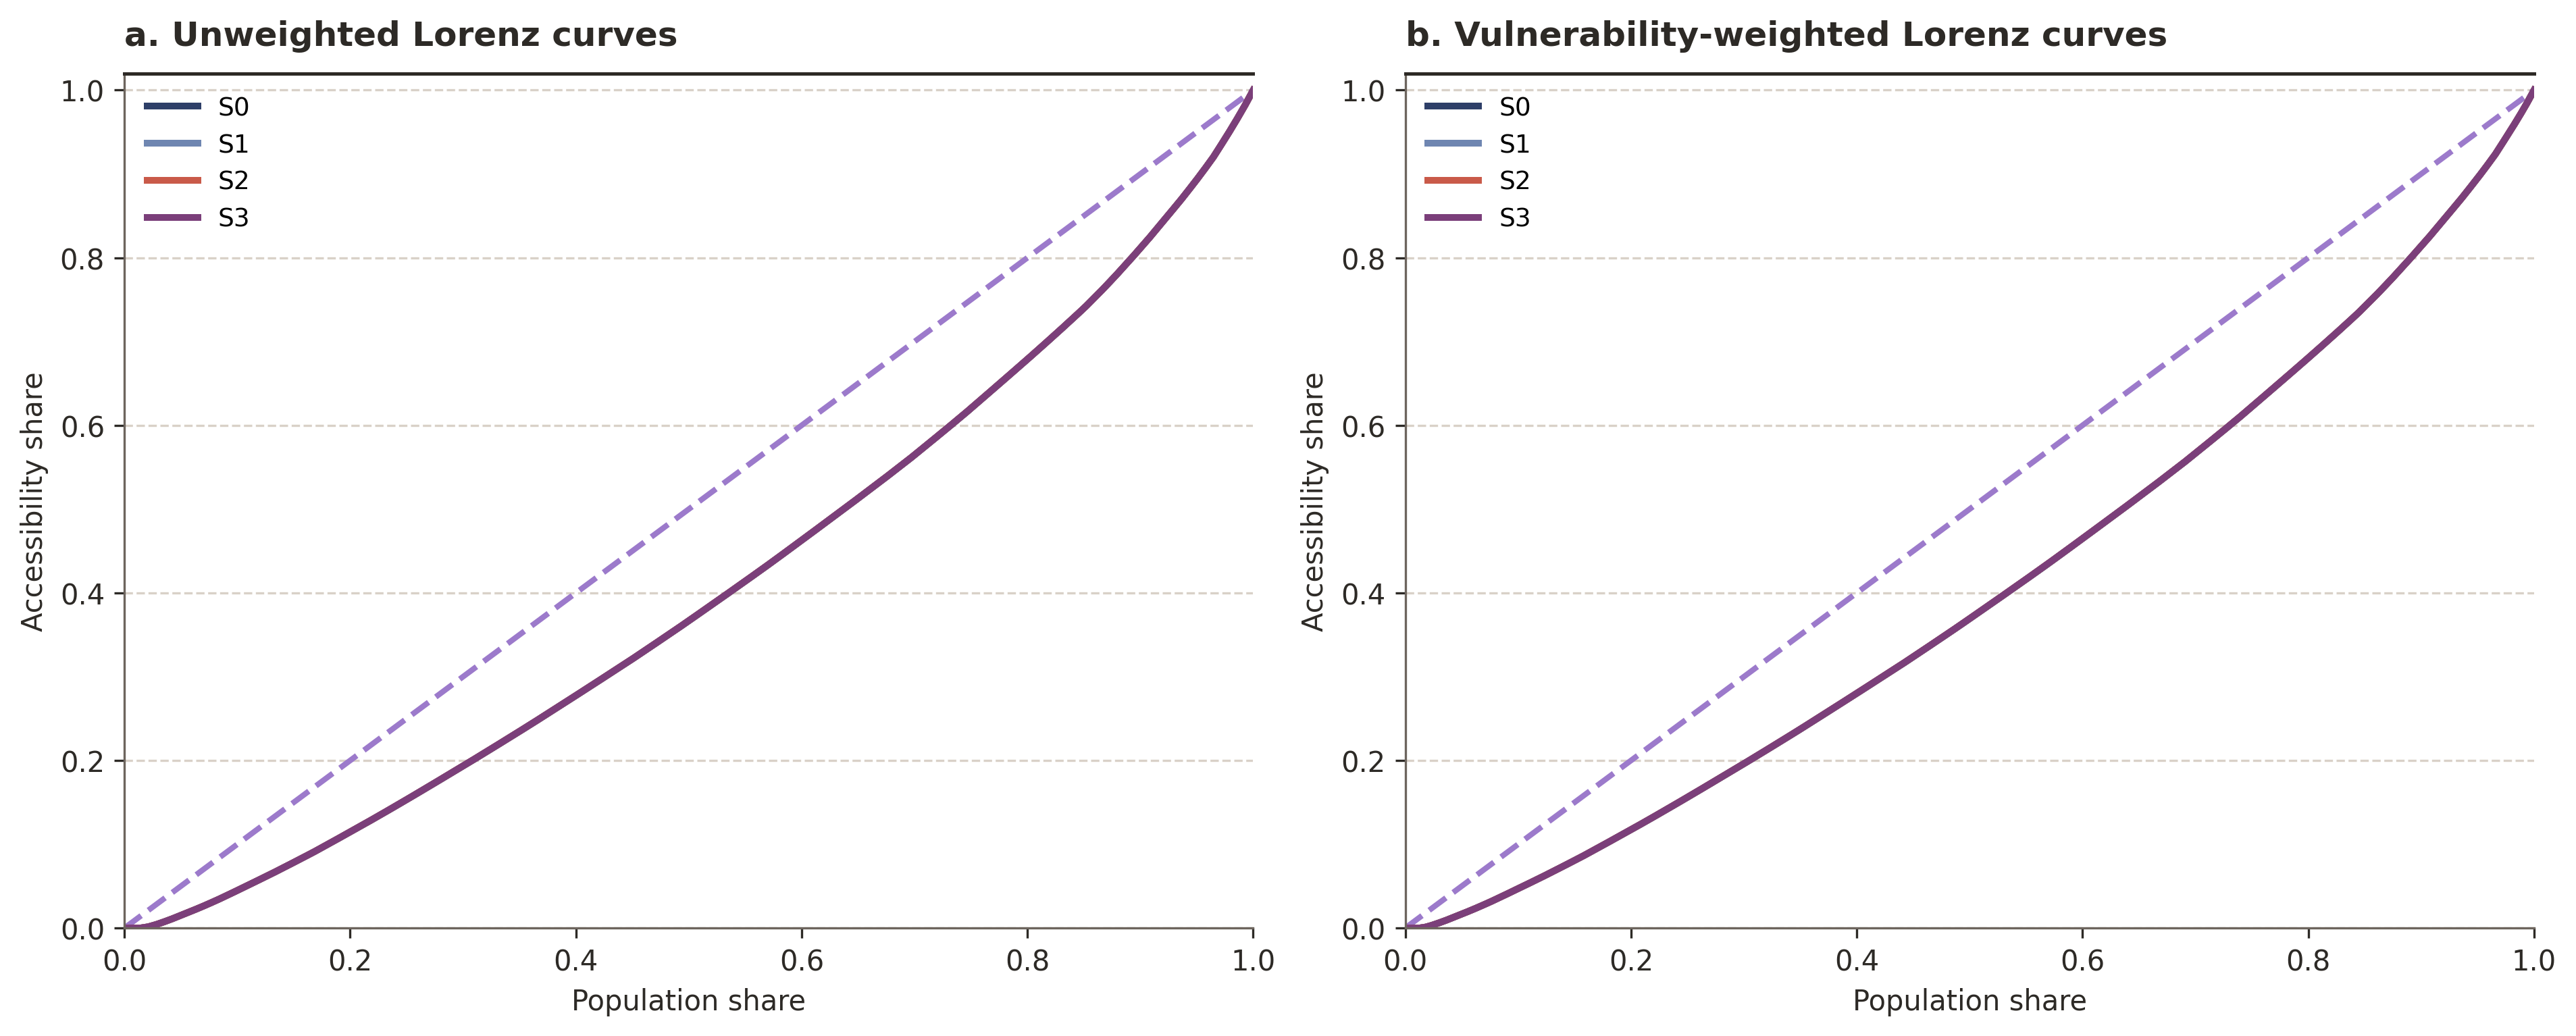
\includegraphics[width=0.98\textwidth]{figures/fig_lorenz_curves.png}
\caption{Unweighted and vulnerability-weighted accessibility Lorenz curves across scenarios.}
\label{fig:lorenz_curves}
\end{figure*}

\begin{table*}[t]
\centering
\caption{Compact policy trade-off summary across scenarios.}
\label{tab:policy_tradeoff}
\begin{threeparttable}
\footnotesize
\begin{tabularx}{\textwidth}{Z Z Z Z Z}
\toprule
Scenario & Objective abs.\ deviation & Fidelity loss vs.\ S0 (\%) & Vulnerable coverage (\%) & Weighted Gini \\
\midrule
S0 & 62.83 & 0.0 & 77.78 & 0.1972 \\
S1 & 64.71 & 3.0 & 86.11 & 0.1970 \\
S2 & 67.85 & 8.0 & 88.89 & 0.1969 \\
S3 & 67.85 & 8.0 & 88.89 & 0.1969 \\
\bottomrule
\end{tabularx}
\begin{tablenotes}[flushleft]
\footnotesize
\item Notes: S2 and S3 overlap exactly in the reproduced run. Relative to S1, the socially weighted scenario lowers the exact weighted Gini from 0.197041 to 0.196896 while changing mean accessibility in $\mathcal{V}^{H}$ from 410.324 to 410.265. The quantitative shift is modest in aggregate terms, but it is generated by only ten one-port reallocations under fixed quotas.
\end{tablenotes}
\normalsize
\end{threeparttable}
\end{table*}

\begin{figure*}[t]
\centering
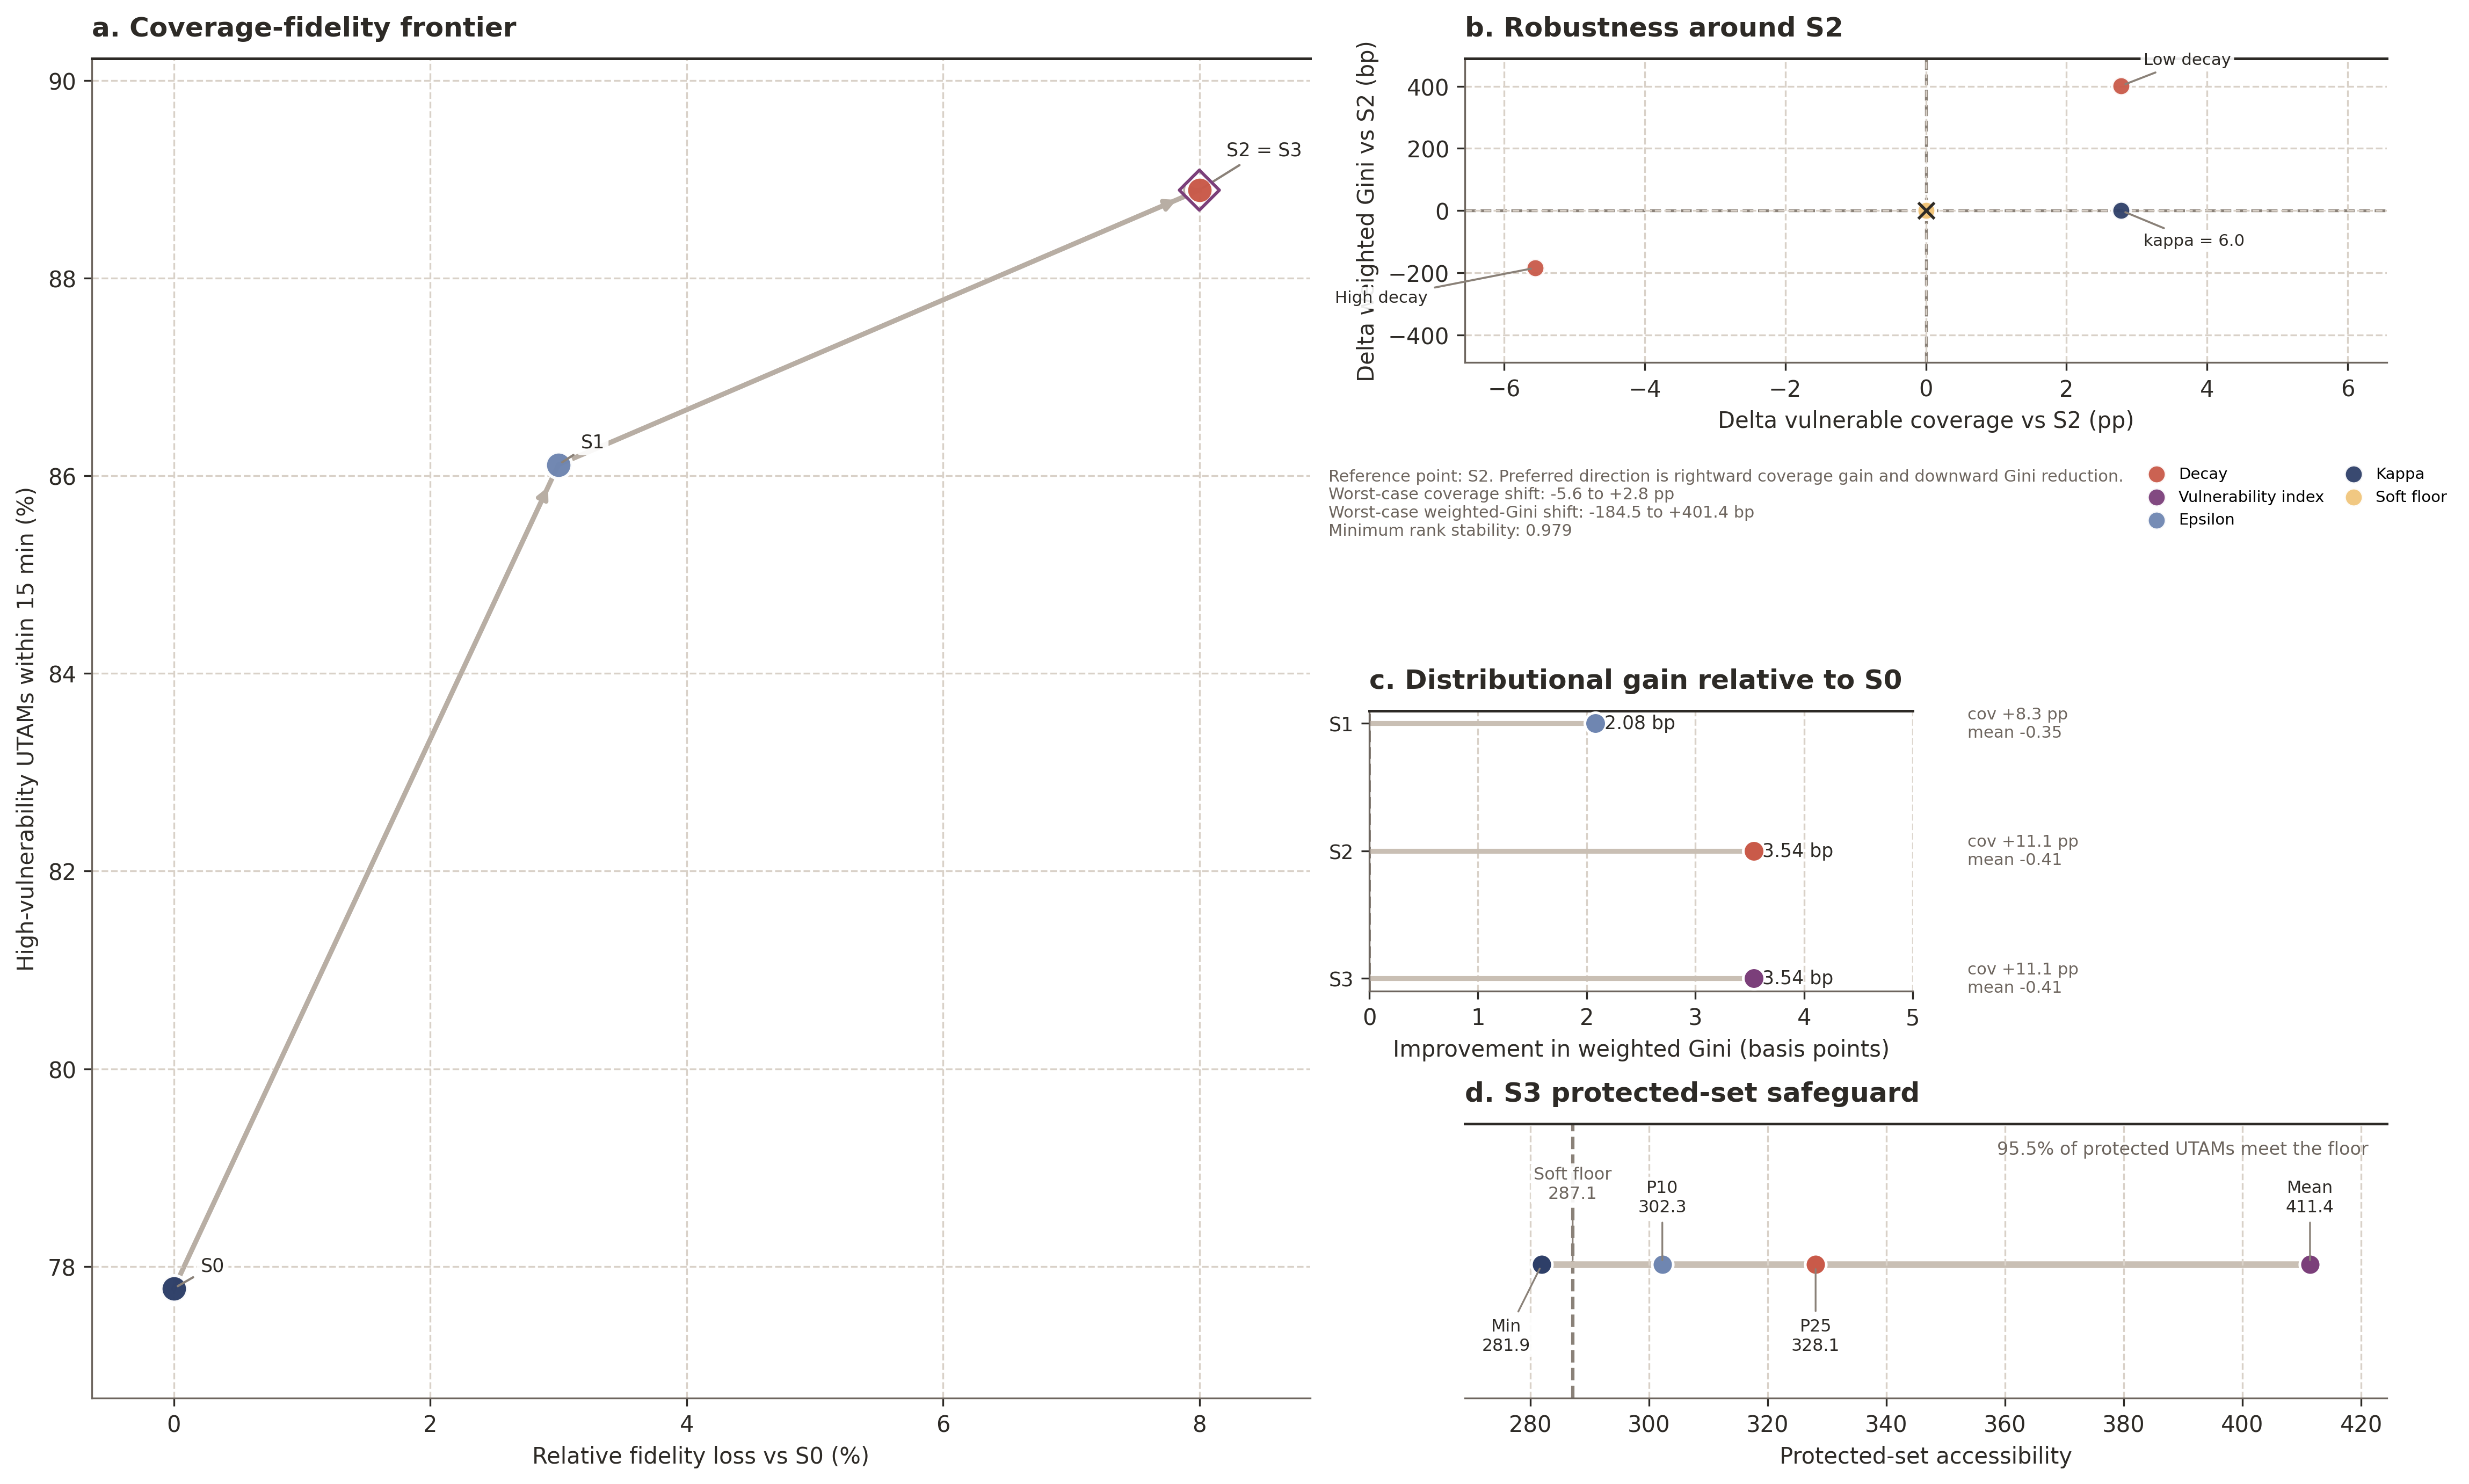
\includegraphics[width=0.98\textwidth]{figures/fig_policy_tradeoff.png}
\caption{Policy trade-off synthesis across allocation scenarios. Panel (a) shows the coverage-fidelity frontier, where the move from S0 to S1 delivers the largest marginal gain in vulnerable-zone coverage and the move from S1 to S2/S3 yields a smaller additional improvement at higher fidelity cost. Panel (b) summarizes robustness around S2 across alternative decay, vulnerability-index, epsilon, kappa and soft-floor specifications. Panel (c) reports weighted-Gini improvements relative to S0 alongside gains in vulnerable coverage and mean accessibility for high-vulnerability areas. Panel (d) reports the lower-tail safeguard for the protected set under S3. S2 and S3 overlap on the frontier because the soft-floor safeguard is non-binding in the reproduced allocation.}
\label{fig:policy_tradeoff}
\end{figure*}

\subsection{Sensitivity and policy robustness checks}

Additional robustness checks indicate that the policy ordering is stable across plausible
specification changes. Relative to the S2 baseline, the Spearman rank correlation of
zone-level total allocated ports remains between 0.9958 and 1.0000 when the vulnerability
index is reconstructed with PCA weights or the lexicographic tolerance varies between 0.056
and 0.100. The main sensitivity comes from the accessibility-decay parameters: relative to
S2, reducing all $\lambda_v$ values by 25\% worsens the weighted Gini by 0.040144 and
raises vulnerable coverage by 2.78 percentage points, whereas increasing them by 25\%
improves the weighted Gini by 0.018454 but lowers vulnerable coverage by 5.56 percentage
points. Even in those cases, the same rank-stability measure remains high (0.9791--0.9839),
so the qualitative scenario ordering is preserved. No alternative travel-time matrix with
sufficient coverage was available for a full comparative rerun, so robustness should be read
as conditional on the reproduced impedance structure.

\section{Discussion}

This study shows that charger planning becomes a transport-geography question once learned
demand signals are evaluated through the spatial distribution of accessibility rather than
through charger counts alone. The reproduced results reveal a clear but bounded trade-off.
Priority-preserving allocation remains closest to the learned mobility surface, whereas
vulnerability weighting redirects a small share of capacity toward zones where households
are less able to rely on private charging. The important empirical result is therefore not a
wholesale remapping of the city, but a selective redistribution within the consolidated
urban core: only 10 zones change, yet vulnerable coverage rises from 86.11\% to 88.89\%
and both weighted and unweighted accessibility inequality decline under fixed quotas.
The aggregate inequality changes are numerically small, but this is exactly what should be
expected when the feasible intervention is a limited set of one-port moves rather than a
continuous reallocation of capacity.

That pattern matters for interpretation. It suggests that mobility-derived priority and
social disadvantage overlap only partially, so equity gains come from rebalancing the lower
tail of accessibility rather than abandoning the main demand geography. The contribution is
thus substantive as well as methodological: it shows how a model trained on observed
mobility can be translated into explicit allocation rules that remain readable to planners,
auditable in policy terms, and sensitive to the uneven geography of charging disadvantage.
For data-constrained cities, the framework remains practical because it relies on surveys,
socioeconomic records, and network travel times rather than charging telemetry.

\subsection{Geographical implications and implementation pathway}

The scenario sequence $S1 \to S2 \to S3$ can still be read as a staged governance pathway,
but the reproduced run sharpens its interpretation. Territorial equalization comes first as
the lowest-friction equity adjustment under fixed quotas. Vulnerability weighting follows
once proxy evidence on charging disadvantage is available and politically defensible. Soft
floors, in turn, operate as monitoring safeguards and auditing devices in the reproduced
configuration; stronger redistributive use would require additional sensitivity analysis over
$\beta$, $\gamma$, and the size of the protected set.

The minimum reproducible data package is modest: zonal mobility indicators, socioeconomic
vulnerability proxies, an OD travel-time matrix, externally defined charger quotas, and a
defensible citywide understanding of EV growth. In Bogot\'a, the official trajectory from
2,039 registered EVs in late 2020 to 8,899 in late 2024 underscores why these allocation
decisions are no longer marginal, even in settings where detailed charging telemetry is not
yet available.

The framework also has limitations. Vulnerability indicators are proxy-based and measured at
the UTAM level, official EV-growth checkpoints are irregular rather than monthly, scenario
outcomes depend on decay and weighting assumptions, and the current setup is static rather
than multi-period. Transferability therefore depends less on reproducing the exact model
architecture than on securing consistent zoning, a defensible travel-time matrix, minimal
vulnerability proxies, externally defined quotas, and institutional capacity to interpret
scenario-based optimization results. Because the article prioritizes the learning-to-decision
translation over algorithmic competition, it also does not present an exhaustive benchmark
contest against simpler forecasting models; the substantive claims should therefore be read
as conditional on the reproduced learning stage rather than as a claim of universal model
superiority.

Overall, the central implication is both methodological and geographical: learning-derived
demand signals become policy-ready only when their translation into optimization parameters is
explicit, auditable, and socially interpretable.

\section{Conclusions}

This paper shows that EV charger planning can move from territorial equalization toward
social equity through a unified learning-and-optimization approach. In the reproduced run,
the socially weighted scenario changes allocations in 10 zones, reduces the
vulnerability-weighted accessibility Gini from 0.197041 to 0.196896, and raises coverage of
vulnerable UTAMs within 15 minutes from 86.11\% to 88.89\%, at an 8.0\% fidelity loss
relative to the priority-matching baseline.

The soft-floor extension is informative as a robustness check but does not change the
reproduced allocation relative to S2: S3 coincides with S2, and 95.45\% of protected zones
already satisfy the calibrated minimum-service floor. For Bogot\'a and
similar data-constrained cities, the practical implication is staged deployment: begin with a
demand-preserving baseline, relax toward territorial equity, add vulnerability weighting when
the proxy evidence is credible, and use soft floors first as monitoring safeguards in the
reproduced configuration, tightening them into stricter service guarantees only after
additional sensitivity analysis.

\section*{Supplementary material}
Notation tables and supplementary figures for graph learning, target extraction,
optimization, equity, and robustness checks are provided in the separate supplementary
appendix submitted with the manuscript.


% CRediT, declaration of competing interests, and acknowledgements are supplied separately
% on the title page to comply with double anonymized review.



\section*{Data availability}
Code, figure-generation scripts, and the shareable processed data and derived non-sensitive
outputs used to reproduce the analysis are archived in a blinded replication package prepared
for double-anonymized review. Repository identifiers are omitted from the manuscript and can
be supplied directly to the editor. The full raw input datasets cannot be deposited publicly
because some sources are subject to licensing, institutional-access, or privacy-related
restrictions.

\bibliographystyle{elsarticle-harv}
\bibliography{data_additional/references_parta}

\end{document}